%*****************************************
\chapter{Presenting Data with Charts}\label{ch04:charts}
%*****************************************
% Second pass corrections made and grammar checked 220622

One of the most important things to consider when using charts in Excel is that they are intended to be used for communicating an idea to an audience, whether that audience is reading a written report or listening to a presentation. Excel charts are often imported or pasted into Word documents or PowerPoint slides, which serve the purpose of communicating ideas to an audience. Although there are no rules set in stone for using specific charts for certain data types, some chart types are designed to communicate specific messages better than others. This chapter explores numerous charts that can be used for various purposes. In addition, the chapter examines formatting charts and using those charts in Word and PowerPoint documents.

\section{Choosing a Chart Type}

\begin{center}
	\begin{objbox}{Learning Objectives}
		\begin{itemize}
			\setlength{\itemsep}{0pt}
			\setlength{\parskip}{0pt}
			\setlength{\parsep}{0pt}

			\item Construct a line chart to show a time series trend.
			\item Learn how to adjust the Y-Axis scale.
			\item Construct a line chart to present a comparison of two trends.
			\item Learn how to use a column chart to show a frequency distribution.
			\item Create a separate chart sheet for a chart embedded in a worksheet.
			\item Construct a column chart that compares two frequency distributions.
			\item Learn how to use a pie chart to show the percent of total for a data set.
			\item Construct a stacked column chart to show how a percent of total changes over time.
			
		\end{itemize}
	\end{objbox}
\end{center}

This section reviews the most used Excel chart types. It is necessary to use a variety of data sets to demonstrate the construction of charts and explain how to choose the right type of chart given the idea being communicated.

Before creating an Excel chart, here are a few key points to consider. 

\begin{itemize}
	\item Identify the idea or message. It is important to remember that a chart's primary purpose is to present quantitative information to an audience. Therefore, first, decide what message or idea is being presented. This chapter continually reinforces the idea of determining the intended message before creating each chart.
	\item Select the right chart type based on the data and the communicated message.
	\item Identify the values that should appear on the X-Axis and Y-Axis. One of the ways to identify which values belong on the axes is to sketch the chart on paper first. Visualizing the chart first makes selecting the information more straightforward, and then using Excel to construct an effective chart that accurately communicates the message. 
\end{itemize}

Table \ref{04:tab01}, \textit{Key Steps Before Constructing an Excel Chart}, summarizes the preceding points.

\begin{table}[H]
	\rowcolors{1}{}{tablerow} % zebra striping background
	{\small
		%\fontsize{8}{10} \selectfont %Replace small for special font size
		\begin{longtable}{L{0.75in}L{3.50in}} %Left-aligned, Max width: 4.25in
			\textbf{Step} & \textbf{Description} \endhead
			\hline
			Define the message & Identify the main idea being communicated. If there is no main point or important message that can be revealed by a chart, then do not create a chart.\\
			Identify the data needed & Once there is a clear message, identify the data on a worksheet needed to construct a chart. In some cases, formulas may be needed to define the data better, or some items may need to be consolidated into broader categories.\\
			Select a chart type & The type of chart selected will depend on the message being communicated and the data being presented.\\
			Identify the values for the X-Axis and Y-Axis & After selecting a chart type, drawing a sketch is often helpful in identifying which values should be on the X-Axis and Y-Axis. In Excel, the axes are the X, or "category," axis, the horizontal axis with labels; and the Y, or "value," axis, the vertical axis with numbers.\\
			\rowcolor{captionwhite}
			\caption{Key Steps before Constructing an Excel Chart}
			\label{04:tab01}
		\end{longtable}
	} % End small
\end{table}

\subsection{Time Series Trend: Line Chart 1}

Figure \ref{04:fig01} shows part of the data that will be used to create two different line charts. The first will show the trend of the NASDAQ stock index\footnote{The NASDAQ data was found at \url{http://www.investopedia.com/terms/n/nasdaq.asp}}.

This chart will communicate a simple message: to show how the index has performed over two years. This chart can be used in a presentation to show whether stock prices have been increasing, decreasing, or remaining constant over the designated period.

\begin{center}
	\begin{infobox}{Integrity Check}
		\textbf{Carefully Select Data When Creating a Chart}
		\\
		\\
		Just because a worksheet contains data does not mean it must all be placed onto a chart. When creating a chart, it is common for only specific data points to be used. To determine what data should be used when creating a chart, start by identifying the message or idea that must be communicated to the audience.
	\end{infobox}
\end{center}

\begin{figure}[H]
	\centering
	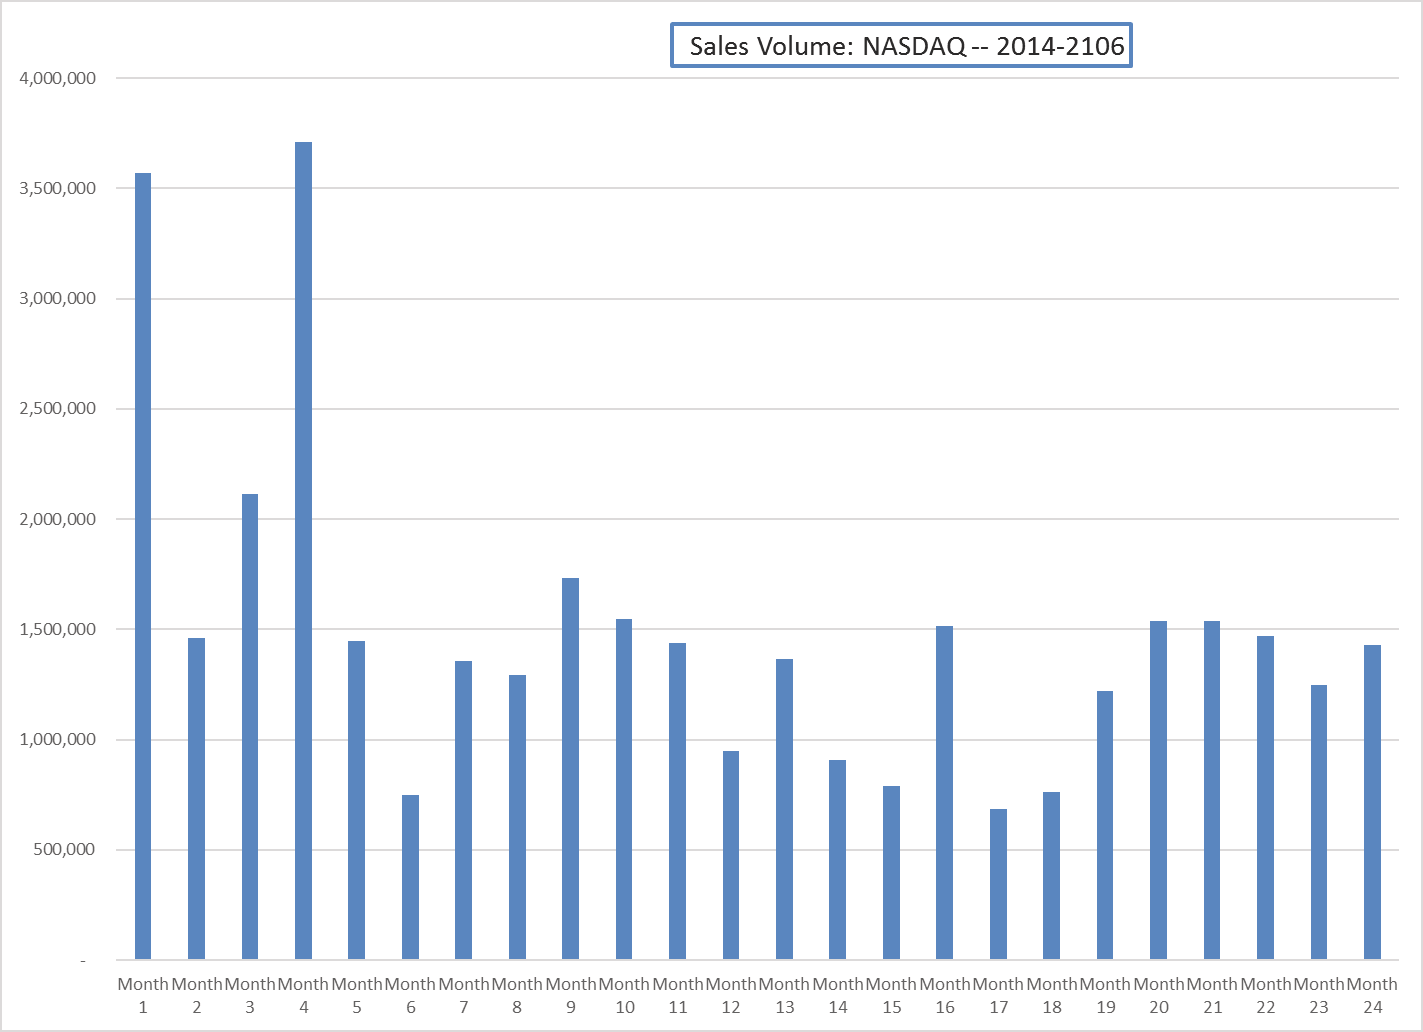
\includegraphics[width=\maxwidth{.95\linewidth}]{gfx/ch04_fig01}
	\caption{Stock Trends}
	\label{04:fig01}
\end{figure}

Before creating the line chart, it is essential to identify why it is an appropriate chart type given the message being communicated and the data available. When presenting the trend for any data over a designated period, the most used chart types are line and column charts. The line chart in this exercise will show the Month number on the X-Axis and the sales volume for the NASDAQ on the Y-Axis. Column charts will be used in later projects.

\begin{enumbox}
	\begin{enumerate}
		\item Open data file \fmtWorksheet{CH4-Data} and save it as \fmtWorksheet{CH4-Charting}.
		\item Open the \fmtWorksheet{Stock Trend} worksheet.
		\item Select \fmtLoc{B4:C28}. (Notice that labels in the \fmtLoc{B4:C4} and all the labels in \fmtLoc{B5:B28} are selected. Observe where they show up in the completed chart.)
		\item Click \fmtButton{Insert $ \Rightarrow $ Charts $ \Rightarrow $ Line Chart Down Arrow $ \Rightarrow $ 2D Line Chart} (this is the first option from the \textit{Line Chart} list, see Figure \ref{04:fig02}).
	\end{enumerate}
\end{enumbox}
	
\begin{figure}[H]
	\centering
	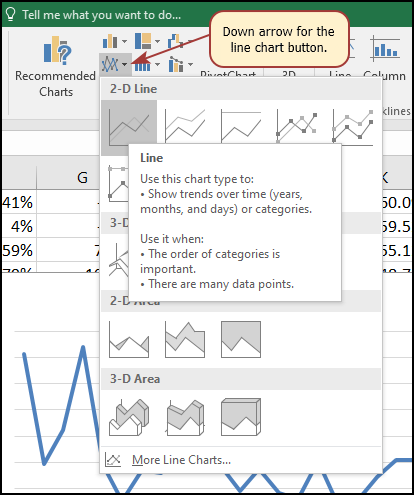
\includegraphics[width=\maxwidth{.85\linewidth}]{gfx/ch04_fig02}
	\caption{Selecting the Basic Line Chart}
	\label{04:fig02}
\end{figure}

The above procedure adds the line chart to the worksheet, as shown in Figure \ref{04:fig03}. Notice where the labels showed up on the chart.

\begin{center}
	\begin{infobox}{Why?}
		\textbf{Line Chart vs. Column Chart}
		\\
		\\
		Both a line chart and a column chart can be used to illustrate a trend over time. However, a line chart is far more effective when there are many periods of time being measured. For example, if fifty-two weeks are being reported a column chart would require fifty-two bars. A general rule of thumb is to use a column chart when twenty bars or fewer are required. A column chart becomes difficult to read as the number of bars exceeds twenty.
	\end{infobox}
\end{center}

Notice that additional ``contextual'' tabs are added to the ribbon when a chart is selected and only appear when the chart is active. The commands in these tabs will be demonstrated throughout this chapter.

\begin{figure}[H]
	\centering
	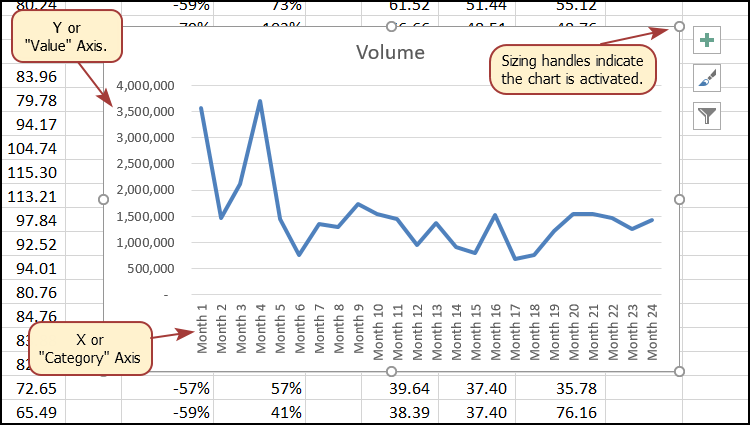
\includegraphics[width=\maxwidth{.95\linewidth}]{gfx/ch04_fig03}
	\caption{Embedded Line Chart in the Stock Trend Worksheet}
	\label{04:fig03}
\end{figure}

As shown in Figure \ref{04:fig03}, the chart is not placed in an ideal location on the worksheet since it covers several cell locations that contain data. The following steps demonstrate standard adjustments when working with charts.

\begin{tabular}{p{3.25in}p{0.5in}} %Max width: 4.25in
	\hline
	\textit{Note for the next step:} The pointer will change into the shape illustrated on the right when it is in the right place to \textbf{move} the chart. & \raisebox{-0.30in}{
\includegraphics[]{gfx/ch04_fig99}} \\
	\hline
	\textit{Note for the next step:} The pointer will change into the shape illustrated on the right when it is in the right place to \textbf{resize} the chart. & \raisebox{-0.30in}{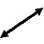
\includegraphics[]{gfx/ch04_fig98}} \\
	\hline
\end{tabular}

\begin{enumbox}
	\begin{enumerate}
		\item Click and drag the chart until its upper left corner is near the top-left corner of cell \fmtLoc{B30}.
		\item Place the mouse pointer over the sizing handle in the upper right corner of the chart, press and hold \fmtKeystroke{Alt}, then left-click and drag that handle until it ``snaps'' to the top of \fmtLoc{Row 30} and the right side of \fmtLoc{Column I}.
		\item Place the mouse pointer over the sizing handle in the lower left corner of the chart, press and hold \fmtKeystroke{Alt}, then left-click and drag that handle until it ``snaps'' to the bottom of \fmtLoc{Row 45} and the left side ``snaps'' to the left side of \fmtLoc{Column B}.
		\item Click the chart title once and then click in front of the first letter. This should place a blinking cursor in front of the letter which allows the title of the chart to be modified. Type the following in front of the first letter in the chart title: \fmtTyping{May 2014-2016 Trend for NASDAQ Sales}.
		\item Click anywhere outside of the chart to deactivate it.
		\item Save the \fmtWorksheet{CH4-Charting} workbook.
	\end{enumerate}
\end{enumbox}
	
Figure \ref{04:fig04} shows the line chart after it is moved and resized. Notice the chart's title is \fmtTyping{May 2014-2016 Trend for NASDAQ Sales Volume}. There are no sizing handles around the chart since it has been deactivated. To activate the chart, click anywhere inside its perimeter.

\begin{figure}[H]
	\centering
	
\includegraphics[width=\maxwidth{.95\linewidth}]{gfx/ch04_fig04}
	\caption{Line Chart Moved and Resized}
	\label{04:fig04}
\end{figure}

\begin{center}
	\begin{sklbox}{Skill Refresher}
		\textbf{Inserting a Line Chart}
		\\
		\begin{itemize}
			\setlength{\itemsep}{0pt}
			\setlength{\parskip}{0pt}
			\setlength{\parsep}{0pt}

			\item Select a range of cells that contain data that will be used to create the chart. Be sure to include labels in the selection.
			\item Click \textit{Insert $ \Rightarrow $ Charts $ \Rightarrow $ Line Chart}. Then, click the icon for the specific type of chart desired.
			
		\end{itemize}
	\end{sklbox}
\end{center}

\begin{center}
	\begin{infobox}{Integrity Check}
		\textbf{Category Axis}
		\\
		\\
		When using line charts in Excel, keep in mind that anything placed on the \textit{X-Axis} is considered a descriptive label, not a numeric value. This is an example of a category axis. This is important because there will never be a change in the spacing of any items placed on the \textit{X-Axis} of a line chart. If numeric data must be placed on the category axis, the chart will need to be modified, which is covered later in the chapter.
	\end{infobox}
\end{center}

\subsubsection{Adjusting the Y-Axis Scale}

After creating an Excel chart, it may be necessary to adjust the scale of the Y-Axis. Excel automatically sets the maximum value for the Y-Axis based on the data used to create the chart, and the minimum value is usually set to zero. That is usually appropriate. However, depending on the data used to create the chart, setting the minimum value to zero can substantially minimize the graphical presentation of a trend. For example, the trend shown in Figure \ref{04:fig04} appears to be increasing slightly in recent months. The trend is easier to notice if the Y-Axis minimum value starts at $ 500,000 $ instead of zero. The following steps explain how to adjust the Y-Axis.

\begin{enumbox}
	\begin{enumerate}
		\item Right-click anywhere on the \textit{Y-Axis} (\textit{Value Axis} or \textit{Vertical Axis}) on the \textit{May 2014-2016 Trend for NASDAQ Sales Volume} line chart in the \fmtWorksheet{Stock Trend} worksheet.
		\item Select \fmtButton{Format Axis} in the pop-up context menu. The \textit{Format Axis} pane should appear on the right side of the screen, as shown in Figure \ref{04:fig05}. \textit{Note}: If \fmtButton{Format Axis} is not on the context menu, the mouse was clicked in the wrong location. Tap \fmtKeystroke{Escape} to turn the menu off and try again.
	
		\begin{figure}[H]
			\centering
			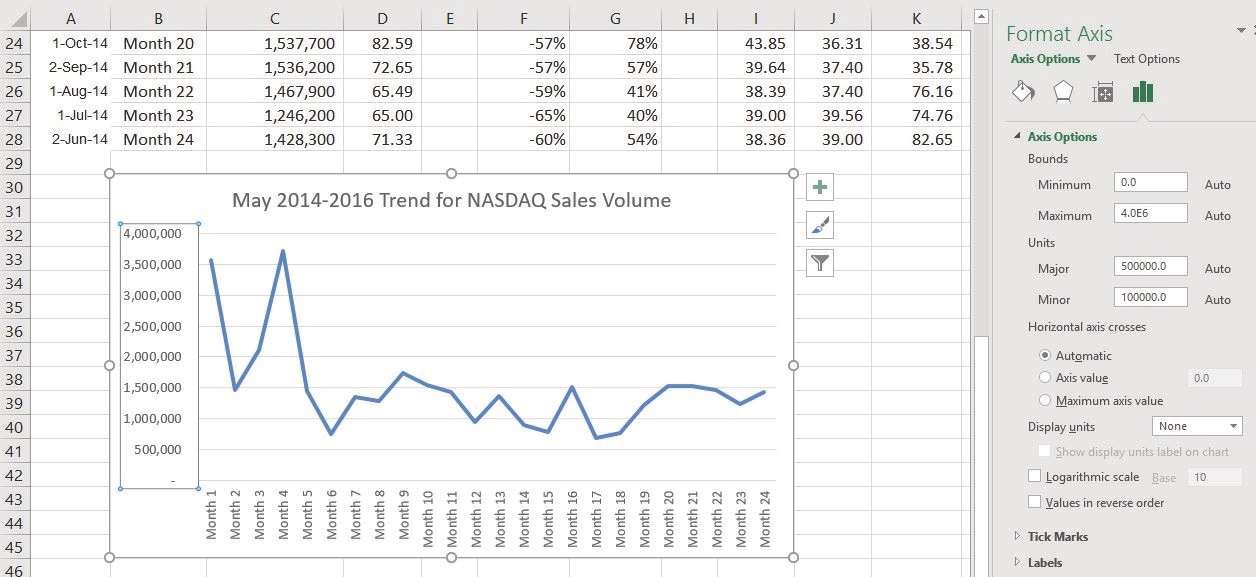
\includegraphics[width=\maxwidth{.95\linewidth}]{gfx/ch04_fig05}
			\caption{Format Axis Pane}
			\label{04:fig05}
		\end{figure}
	
		\item In the \textit{Format Axis} pane, click the input box for the \textit{Minimum} axis option and delete the content of that box. Then type the number $ 500000 $ and tap \fmtKeystroke{Enter}. As soon as this change is made, the Y-Axis on the chart adjusts.
		\item Click the \fmtButton{X} in the upper right corner of the \textit{Format Axis} pane to close it.
		\item Save the \fmtWorksheet{CH4-Charting} workbook.
	\end{enumerate}
\end{enumbox}
	
Figure \ref{04:fig06} shows the change in the presentation of the trend line. Notice that with the Y-Axis starting at $ 500,000 $, the trend for the NASDAQ is more pronounced. This adjustment makes it easier for the reader to see the magnitude of the trend. Do be careful when adjusting the Y-Axis. Adjusting the minimum or maximum of this axis makes it easy to exaggerate a relatively small trend disproportionately.

\begin{figure}[H]
	\centering
	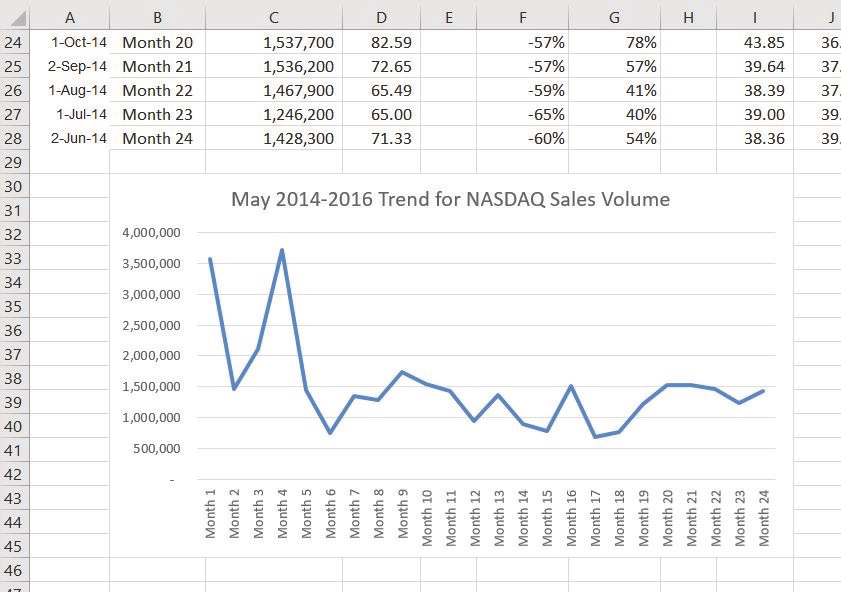
\includegraphics[width=\maxwidth{.95\linewidth}]{gfx/ch04_fig06}
	\caption{Adjusted Y-Axis for the S\&P 500 Chart}
	\label{04:fig06}
\end{figure}

\begin{center}
	\begin{sklbox}{Skill Refresher}
		\textbf{Adjusting the Y-Axis Scale}
		\\
		\begin{itemize}
			\setlength{\itemsep}{0pt}
			\setlength{\parskip}{0pt}
			\setlength{\parsep}{0pt}

			\item Right-click anywhere along the Y-Axis to pop-up the context menu.
			\item Select \textit{Format Axis} where changes can be made to the axis.
			\item Enter the desired amounts for the \textit{Minimum} or \textit{Maximum} values.
			\item Click the \textit{Close} button at the top right of the \textit{Format Axis} pane to close it.
			
		\end{itemize}
	\end{sklbox}
\end{center}

\subsection{Trend Comparisons: Line Chart 2}

A second line chart will be created using the data in the \textit{Stock Trend} worksheet. The purpose of this chart is to compare two trends: the change in \textit{NASDAQ Volume} and \textit{Closing Price}.

Before creating the chart to compare the \textit{NASDAQ Volume} and \textit{Closing Price}, it is essential to review the data in $ B4 $:$ D28 $ on the \textit{Stock Trend} worksheet. Even a brief examination reveals that the \textit{NASDAQ Volume} and \textit{Closing Price} cannot be used directly on the same chart because the values are not comparable. The \textit{NASDAQ Volume} ranges from $ 684,000 $ to $ 3,711,000 $, but the \textit{Closing Price} ranges from $ \$45.00 $ to $ \$115.00 $. If these values are used without scaling, the \textit{Closing Price} would not be visible compared to the \textit{NASDAQ Volume}.

Constructing the second line chart will be like the first. The X-Axis will be the month numbers in $ B4 $:$ D28 $.

\begin{enumbox}
	\begin{enumerate}
		\item Select \fmtLoc{B4:D28} on the \fmtWorksheet{Stock Trend} worksheet.
		\item Click \fmtButton{Insert $ \Rightarrow $ Charts $ \Rightarrow $ Line Chart Down Arrow $ \Rightarrow $ 2D Line Chart} (this is the first option from the \textit{Line Chart} list).
	\end{enumerate}
\end{enumbox}
	
Figure \ref{04:fig07} shows the appearance of the line chart comparing the \textit{NASDAQ Volume} to the \textit{Closing Price} before it is moved and resized. Notice that the red line for \textit{Closing Price} (labeled as \textit{Close} in the legend) appears as a straight line at the bottom of the chart. Also, the chart is so large that it covers the data, and the title needs to be changed.

\begin{figure}[H]
	\centering
	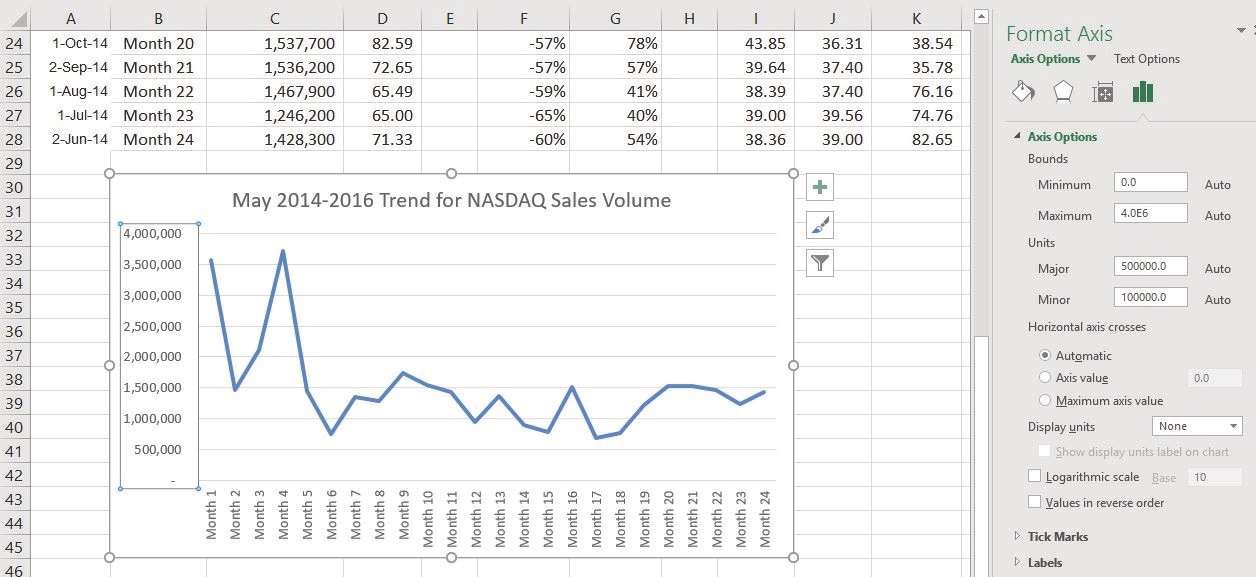
\includegraphics[width=\maxwidth{.95\linewidth}]{gfx/ch04_fig07}
	\caption{Trend Comparison Line Chart}
	\label{04:fig07}
\end{figure}

\begin{enumbox}
	\begin{enumerate}
		\item Move the chart, so the upper left corner is in the middle of cell \fmtLoc{M3}.
		\item Resize the chart using the following values. For each side of the chart, press and hold \fmtKeystroke{Alt}, then left-click and drag the resize handle on the chart to make it ``lock into'' position.
		
		\begin{table}[H]
			\rowcolors{1}{}{tablerow} % zebra striping background
			\captionsetup{labelformat=empty} % kill the label and caption area
			{\small
				%\fontsize{8}{10} \selectfont %Replace small for special font size
				\begin{longtable}{R{0.75in}L{1.50in}} %Left-aligned, Max width: 4.25in
					\textbf{Chart Side} & \textbf{Locked To} \endhead
					\hline
					Top & Top of \fmtLoc{Row 3}\\
					Left & Left of \fmtLoc{Column M}\\
					Bottom & Bottom of \fmtLoc{Row 17}\\
					Right & Right of \fmtLoc{Column U}\\
				\end{longtable}
			} % End small
		\end{table}

		\item Edit the \textit{Chart Title} text box and replace the contents with \fmtTyping{24 Month Trend Comparison}.
	\end{enumerate}
\end{enumbox}

The \textit{Closing Price} data is just a flat red line at the bottom of the chart and cannot be seen very well. Since the chart scale ranges from $ 0 $ to $ 4,000,000 $, the \textit{Closing Price} data is highly compressed. Complete the following steps to add a secondary axis to correct this problem.

\begin{enumbox}
	\begin{enumerate}
		\item Right-click the red line at the bottom of the chart that represents the \textit{Closing Price}.
		\item On the pop-up context menu, select \fmtButton{Format Data Series} to open the \textit{Format Data Series} pane.
		\item In the \textit{Series} Options, select \fmtButton{Secondary Axis}.
	\end{enumerate}
\end{enumbox}
	
\begin{figure}[H]
	\centering
	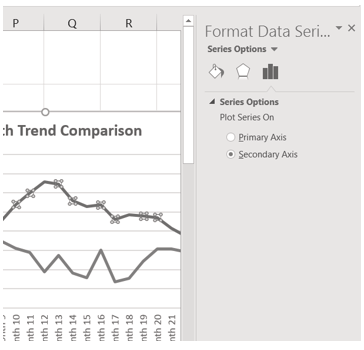
\includegraphics[width=\maxwidth{.75\linewidth}]{gfx/ch04_fig08}
	\caption{Adding a Secondary Axis}
	\label{04:fig08}
\end{figure}

The secondary axis improves the chart, but its numbers should indicate dollar values rather than volume.

\begin{enumbox}
	\begin{enumerate}
		\item Right-click the Secondary Vertical Axis. (The vertical axis on the right that goes from $ 0 $ to $ 140 $.)
		\item From the context menu, select \fmtButton{Format Axis}.
		\item In \textit{Axis Options}, select \fmtButton{Number}. (The menu may need to be scrolled down.)
		\item Use the \textit{Symbol} list box to add the \$ (see Figure \ref{04:fig09}).
		\item Tap \fmtButton{X} (\textit{close}) to close the \textit{Format Axis} pane.
		\item Save the \fmtWorksheet{CH4-Charting} worksheet.
	\end{enumerate}
\end{enumbox}
	
\begin{figure}[H]
	\centering
	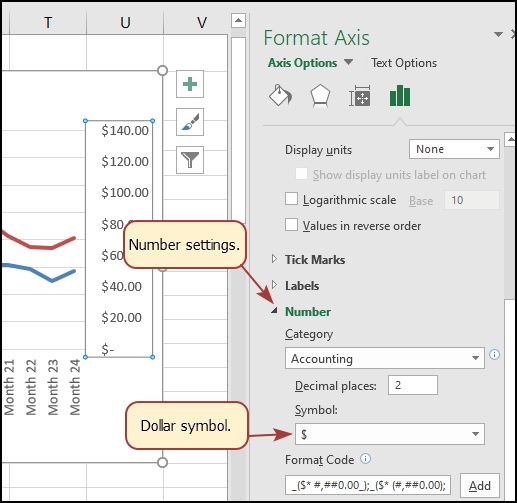
\includegraphics[width=\maxwidth{.75\linewidth}]{gfx/ch04_fig09}
	\caption{Modifying the Secondary Axis}
	\label{04:fig09}
\end{figure}

The chart makes it easy to compare the sales volume with the closing price.

\begin{figure}[H]
	\centering
	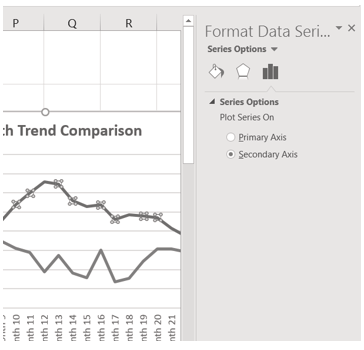
\includegraphics[width=\maxwidth{.95\linewidth}]{gfx/ch04_fig10}
	\caption{Final Comparison Line Chart}
	\label{04:fig10}
\end{figure}

\subsection{``Instant'' Chart – F11}

Excel includes an \textit{Instant Chart} capability that makes charts easy to add with only a few mouse clicks. While these charts may need to be adjusted somewhat, they are often ready to use without additional work. Follow these steps to add an ``instant'' chart. (\textit{NOTE: instant charts are only available if \fmtKeystroke{F11} has not been remapped to a new feature.})

\begin{enumbox}
	\begin{enumerate}
		\item Select \fmtLoc{A4:A28} on the \fmtWorksheet{Stock Trend} worksheet.
		\item Press and hold \fmtKeystroke{Ctrl}, then select \fmtLoc{D4:D28}. Figure \ref{04:fig11} shows the top of the two selected columns.
	
		\begin{figure}[H]
			\centering
			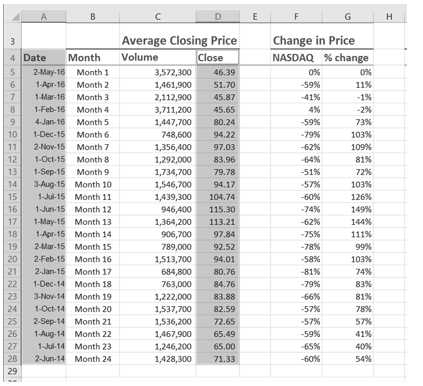
\includegraphics[width=\maxwidth{.65\linewidth}]{gfx/ch04_fig11}
			\caption{Range Selection}
			\label{04:fig11}
		\end{figure}
	
		\item Tap \fmtKeystroke{F11}. If the factory default settings have not been changed, Excel will create a column chart and place it on a separate chart sheet, as illustrated in Figure \ref{04:fig12}.
		\item Change the name of the new worksheet by double-clicking its name: \fmtWorksheet{Chart1}. Type \fmtTyping{Closing Prices} as the new name and tap \fmtKeystroke{Enter}.
		\item Save the \fmtWorksheet{CH4-Charting} workbook.
	\end{enumerate}
\end{enumbox}
	
\begin{figure}[H]
	\centering
	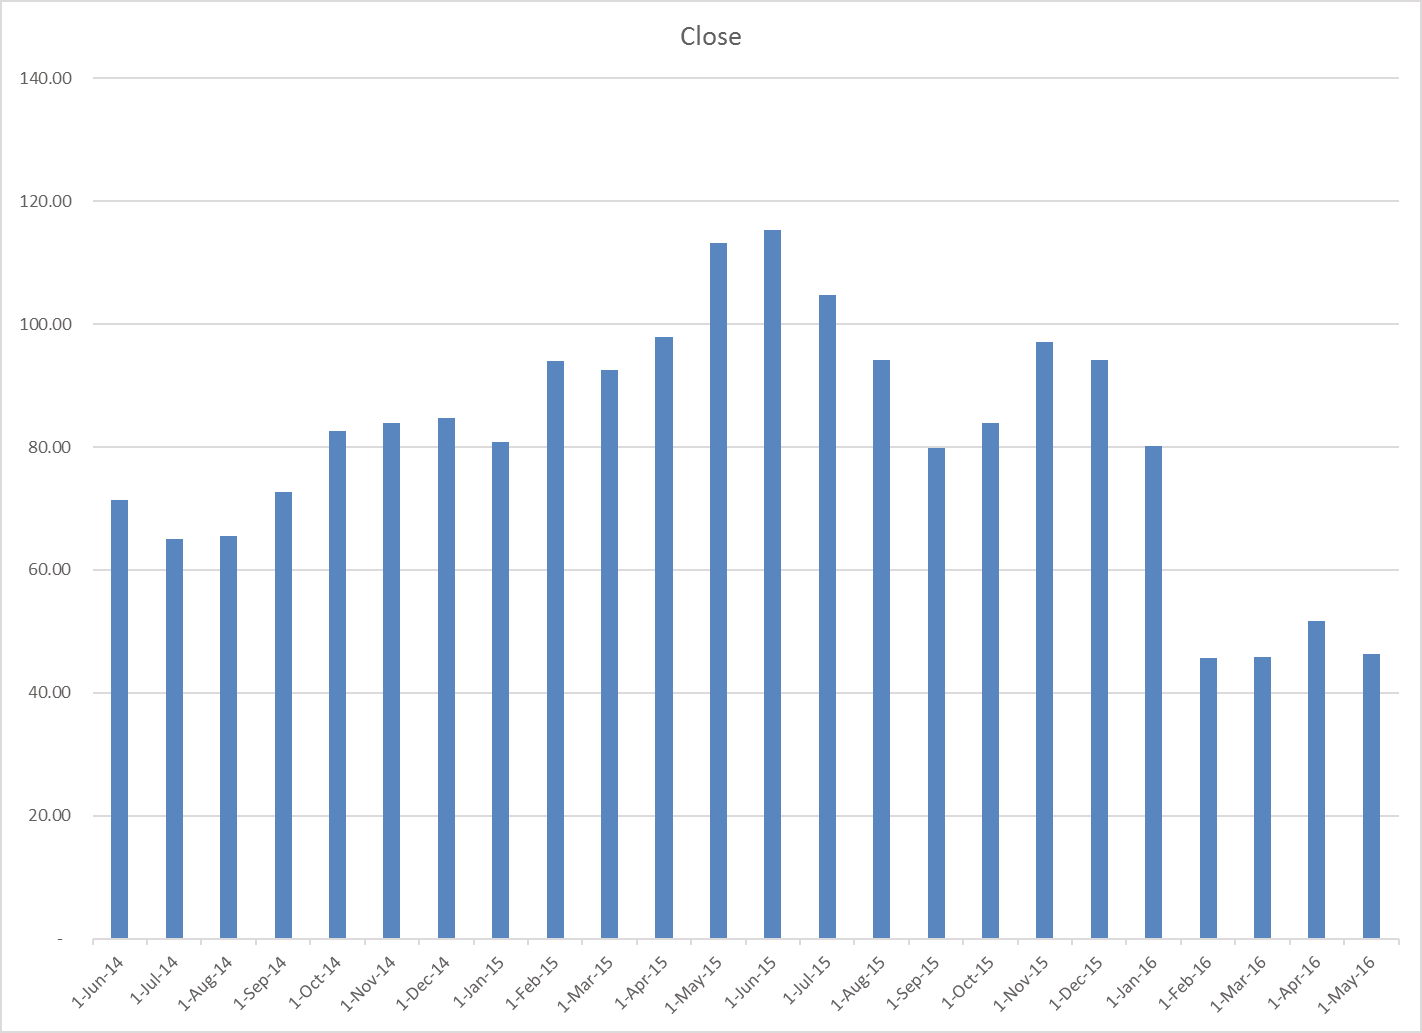
\includegraphics[width=\maxwidth{.95\linewidth}]{gfx/ch04_fig12}
	\caption{Instant Chart}
	\label{04:fig12}
\end{figure}

\subsection{Frequency Distribution: Column Chart 1}

Column charts display a frequency distribution, showing the number of observed occurrences by category. For example, a frequency distribution used in most academic institutions is a grade distribution, which charts the number of students achieving each level of a  grading scale, like A, B, C, and D. The \textit{Grade Distribution} worksheet contains final grades for several hypothetical Excel classes. To show the grade frequency distribution for all the Excel classes in that year, the numbers of students appear on the Y-Axis, and the grade categories appear on the X-Axis. The number of students for this chart is in \textit{Column C}. The labels for grades are in \textit{Column A}. The following steps explain how to create the chart.

\begin{enumbox}
	\begin{enumerate}
		\item Click the \fmtWorksheet{Grade Distribution} worksheet to activate it.
		\item Change the years in \fmtLoc{Row 3} to the current academic term and year.
		\item Select \fmtLoc{A3:A8}, which shows the grade categories.
		\item Tap \fmtKeystroke{Crtl}, then select \fmtLoc{C3:C8}
		\item Click \fmtButton{Insert $ \Rightarrow $ Charts $ \Rightarrow $ Column $ \Rightarrow $ Clustered Column} (this is the first option in the \textit{2-D Column} section).
		
		\begin{figure}[H]
			\centering
			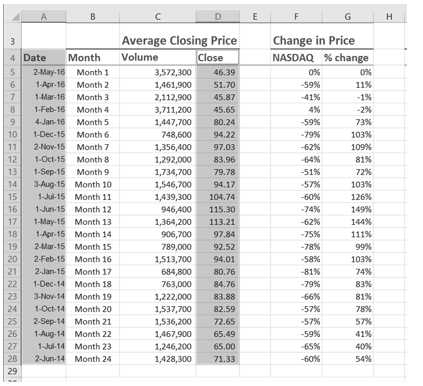
\includegraphics[width=\maxwidth{.65\linewidth}]{gfx/ch04_fig13}
			\caption{Selecting a Column Chart}
			\label{04:fig13}
		\end{figure}
			
		\item Click and drag the chart so the upper left corner is in the middle of cell \fmtLoc{H2}.
		\item Resize the chart using the following values. For each side of the chart, press and hold \fmtKeystroke{Alt}, then left-click and drag the resize handle on the chart to make it ``lock into'' position.
	
		\begin{table}[H]
		\rowcolors{1}{}{tablerow} % zebra striping background
		\captionsetup{labelformat=empty} % kill the label and caption area
		{\small
			%\fontsize{8}{10} \selectfont %Replace small for special font size
			\begin{longtable}{R{0.75in}L{1.50in}} %Left-aligned, Max width: 4.25in
				\textbf{Chart Side} & \textbf{Locked To} \endhead
				\hline
				Top & Top of \fmtLoc{Row 2}\\
				Left & Left of \fmtLoc{Column H}\\
				Bottom & Bottom of \fmtLoc{Row 10}\\
				Right & Right of \fmtLoc{Column O}\\
			\end{longtable}
		} % End small
		\end{table}
	
		\item Excel may have automatically created a legend with the chart, but since it presents only one data series, a legend is unnecessary. Click it one time and tap \fmtKeystroke{Delete} to remove it. 
		\item Add the text \fmtTyping{Final Grades for} to the beginning of the chart title. The chart title should now be \fmtTyping{Final Grades for All Excel Classes 2020/2021} (or whichever academic year is used).
		\item Click any cell location on the \fmtWorksheet{Grade Distribution} worksheet to deactivate the chart.
		\item Save the \fmtWorksheet{CH4-Charting} workbook.
	\end{enumerate}
\end{enumbox}
	
Figure \ref{04:fig14} shows the completed grade frequency distribution chart. Looking at the chart, it is evident that most students earned a final grade in the B+ to B- range.

\begin{figure}[H]
	\centering
	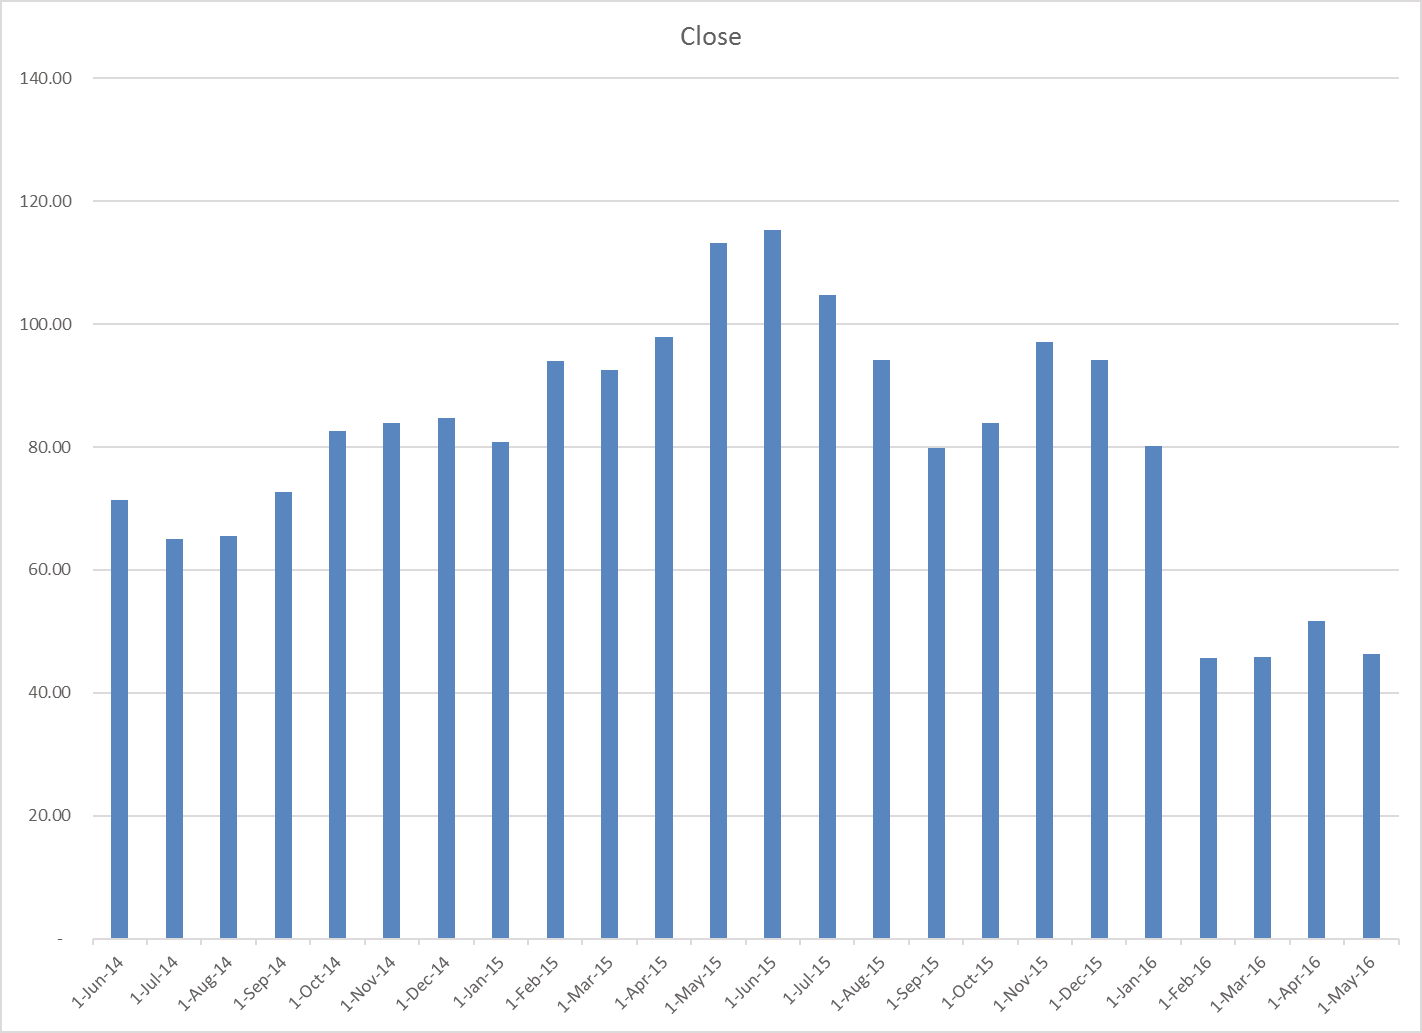
\includegraphics[width=\maxwidth{.95\linewidth}]{gfx/ch04_fig14}
	\caption{Grade Frequency Distribution Chart}
	\label{04:fig14}
\end{figure}

\subsection{Creating a Chart Sheet}

The charts created up to this point have been added to, or embedded in, an existing worksheet (except the \fmtButton{Instant Chart}). Charts can also be placed in a dedicated worksheet called a \textit{chart sheet} because it contains only an Excel chart. Chart sheets are more accessible than having multiple charts embedded in a single worksheet. The following steps explain how to move the grade frequency distribution chart to a dedicated chart sheet.

\begin{enumbox}
	\begin{enumerate}
		\item Right-click anywhere near the edge of the \textit{Final Grades for All Excel Classes} chart on the \fmtWorksheet{Grade Distribution} worksheet.
		\item Select \fmtButton{Move Chart}, which opens the \textit{Move Chart} Dialog box.
		\item Click the \fmtButton{New sheet} option on the \textit{Move Chart} dialog box. (The top option.)
		\item The input box for assigning a chart sheet name is selected when \fmtButton{New Sheet} is clicked. Type \fmtTyping{All Excel Classes}. This replaces the generic name in the input box (see Figure \ref{04:fig15}).
		\item Click the \fmtButton{OK} button at the bottom of the \textit{Move Chart} dialog box. This adds a new chart sheet to the workbook with the name \textit{All Excel Classes}.
		\item Save the \fmtWorksheet{CH4-Charting} workbook.
	\end{enumerate}
\end{enumbox}
	
\begin{figure}[H]
	\centering
	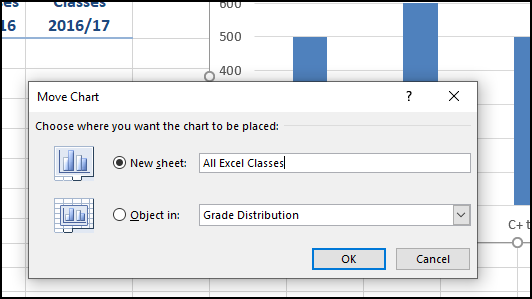
\includegraphics[width=\maxwidth{.95\linewidth}]{gfx/ch04_fig15}
	\caption{Moving a Chart to a Chart Sheet}
	\label{04:fig15}
\end{figure}

\begin{center}
	\begin{infobox}{Why?}
		\textbf{Column Chart vs. Bar Chart}
		\\
		\\
		When using charts to show frequency distributions, the difference between a column chart (where the bars are vertical) and a bar chart (where the bars are horizontal) is really a matter of preference. Both are effective in showing frequency distributions. However, to show a trend over a period of time, a column chart is preferred because a period is typically shown on a horizontal axis, with the oldest date on the left edge and the newest date on the right edge.
	\end{infobox}
\end{center}

Figure \ref{04:fig16} shows the \textit{Final Grades for all Excel Classes} column chart in a separate sheet. Notice that the new worksheet tab added to the workbook matches the name entered into the \textit{Move Chart} dialog box. Since the chart has been moved to a separate chart sheet, it is no longer displayed in the \textit{Grade Distribution} worksheet.

\begin{figure}[H]
	\centering
	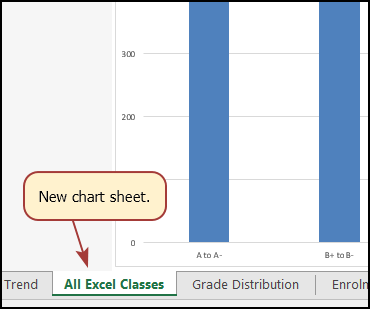
\includegraphics[width=\maxwidth{.65\linewidth}]{gfx/ch04_fig16}
	\caption{Chart Sheet Added to the Workbook}
	\label{04:fig16}
\end{figure}

\subsection{Frequency Comparison: Column Chart 2}

A second column chart will be created to show a comparison between two frequency distributions. \textit{Column B} on the \textit{Grade Distribution} worksheet contains data showing the number of students who received grades within each category for the Spring Quarter. This column chart will compare the grade distribution for Spring (\textit{Column B}) with the overall grade distribution for the whole year (\textit{Column C}). However, since the number of students in the term is significantly different from the total number of students in the year, a percentage must be calculated to make an effective comparison. The following steps explain how to calculate the percentages.

\begin{enumbox}
	\begin{enumerate}
		\item Click the \fmtWorksheet{Grade Distribution} tab to activate that worksheet.
		\item Select \fmtLoc{B9:C9}.
		\item Click \fmtButton{Home $ \Rightarrow $ Editing $ \Rightarrow $ AutoSum}. This automatically adds \fmtButton{SUM} functions that sum the values in \fmtLoc{B4:B8} and \fmtLoc{C4:C8}.
		\item Click \fmtLoc{E4}.
		\item Enter a formula that divides the value in cell \fmtLoc{B4} by the total in cell \fmtLoc{B9}. Add an absolute reference to cell \fmtLoc{B9} in the formula, like this \fmtTyping{=B4/\$B\$9}.
		\item Copy the formula in cell \fmtLoc{E4} and paste it into \fmtLoc{E5:E8} using the Paste command or with \textit{AutoFill}.
		\item Click \fmtLoc{F4}.
		\item Enter a formula that divides the value in cell \fmtLoc{C4} by the total in cell \fmtLoc{C9}. Add an absolute reference to cell \fmtLoc{C9} in the formula, like this \fmtTyping{=C4/\$C\$9}.
		\item Copy the formula in cell \fmtLoc{F4} and paste it into \fmtLoc{F5:F8} using the Paste command or \textit{AutoFill}.
	\end{enumerate}
\end{enumbox}
	
Figure \ref{04:fig17} shows the completed percentages added to the \textit{Grade Distribution} worksheet.

\begin{figure}[H]
	\centering
	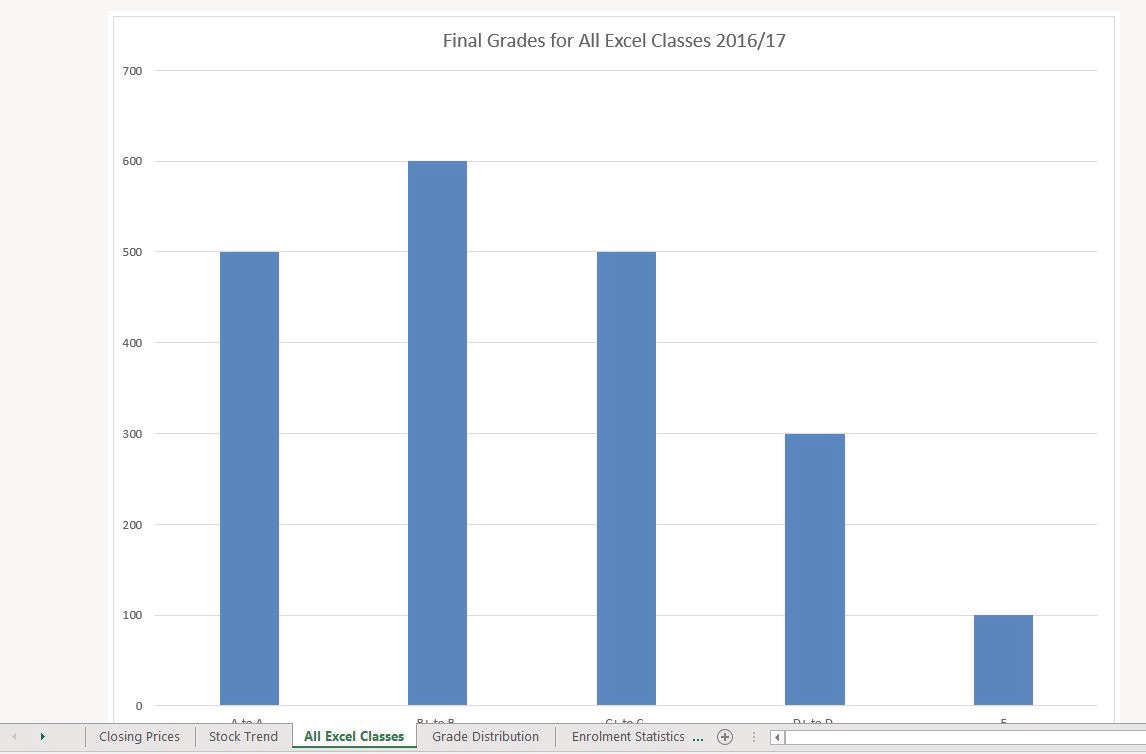
\includegraphics[width=\maxwidth{.95\linewidth}]{gfx/ch04_fig17}
	\caption{Completed Grade Distribution Percentages}
	\label{04:fig17}
\end{figure}

Next, create a column chart that uses the grade categories in $ A4 $:$ A8 $ on the X-Axis and the percentages in $ E4 $:$ F8 $ on the Y-Axis. 

\begin{enumbox}
	\begin{enumerate}
		\item Select \fmtLoc{A3:A8}.
		\item Press and hold \fmtKeystroke{Ctrl}, then select \fmtLoc{E3:F8}.
		\item Click \fmtButton{Insert $ \Rightarrow $ Charts $ \Rightarrow $ Column}. Select the first option from the drop-down list of chart formats, which is the \textit{2-D Clustered Column}.
		\item Click and drag the chart, so the upper left corner is in the middle of cell \fmtLoc{H2}.
		\item Resize the chart using the following values. For each side of the chart, press and hold \fmtKeystroke{Alt}, then left-click and drag the resize handle on the chart to make it ``lock into'' position.
	
		\begin{table}[H]
		\rowcolors{1}{}{tablerow} % zebra striping background
		\captionsetup{labelformat=empty} % kill the label and caption area	
		{\small
			%\fontsize{8}{10} \selectfont %Replace small for special font size
			\begin{longtable}{R{0.75in}L{1.50in}} %Left-aligned, Max width: 4.25in
				\textbf{Chart Side} & \textbf{Locked To} \endhead
				\hline
				Top & Top of \fmtLoc{Row 2}\\
				Left & Left of \fmtLoc{Column H}\\
				Bottom & Bottom of \fmtLoc{Row 10}\\
				Right & Right of \fmtLoc{Column N}\\
			\end{longtable}
		} % End small
		\end{table}
	
		\item Change the chart title to \fmtTyping{Grade Distribution Comparison}. To add a chart title if one is not present, click \fmtButton{Chart Tools Design $ \Rightarrow $ Chart Layouts $ \Rightarrow $ Add Chart Element $ \Rightarrow $ Chart Title $ \Rightarrow $ Above Chart}.
		\item Save the \fmtWorksheet{CH4-Charting} workbook.
	\end{enumerate}
\end{enumbox}

Figure \ref{04:fig18} shows the completed data series operation.

\begin{figure}[H]
	\centering
	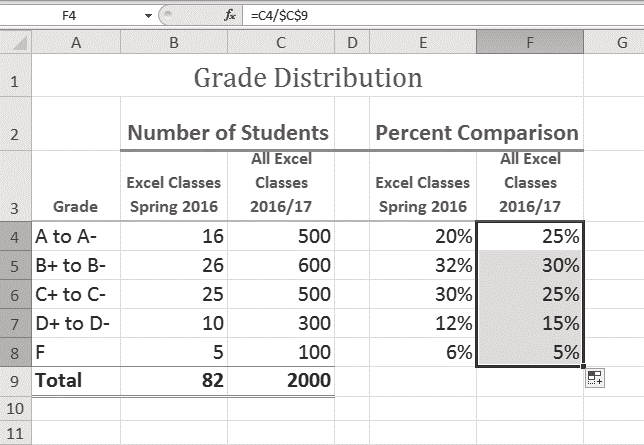
\includegraphics[width=\maxwidth{.95\linewidth}]{gfx/ch04_fig18}
	\caption{Completed Data Series for the Class Grade Distribution}
	\label{04:fig18}
\end{figure}

Figure \ref{04:fig19} shows the final appearance of the column chart. The column chart is appropriate for this data because there are fewer than twenty data points, and it is easy to compare each category. A reader can quickly see that the spring class issued fewer \textit{A's} than the rest of the academic year but more \textit{B's} and \textit{C's}.

\begin{figure}[H]
	\centering
	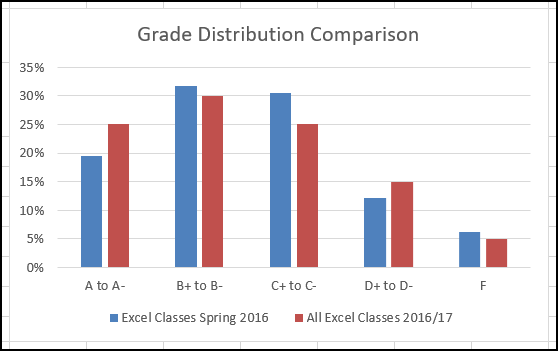
\includegraphics[width=\maxwidth{.95\linewidth}]{gfx/ch04_fig19}
	\caption{Completed Grade Distribution Column Chart}
	\label{04:fig19}
\end{figure}

\begin{center}
	\begin{infobox}{Integrity Check}
		\textbf{Too Many Bars on a Column Chart?}
		\\
		\\
		 Although there is no specific limit for the number of bars used on a column chart, a general rule of thumb is twenty bars or less. Figure \ref{04:fig20} contains a total of thirty-two bars. This is considered a poor use of a column chart because it is difficult to identify meaningful trends or comparisons. The data used to create this chart might be better used in two or three different column charts, each with a distinct idea or message.
	\end{infobox}
\end{center}

\begin{figure}[H]
	\centering
	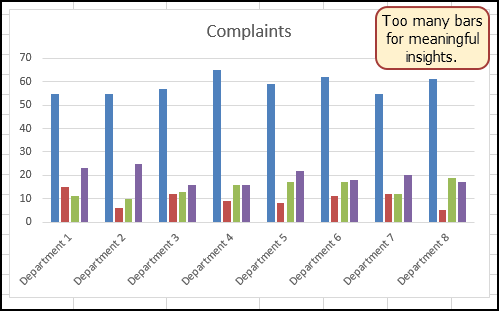
\includegraphics[width=\maxwidth{.95\linewidth}]{gfx/ch04_fig20}
	\caption{Poor Use of a Column Chart}
	\label{04:fig20}
\end{figure}

\subsection{Percent of Total: Pie Chart}

A pie chart shows a percent of the total for a data set at a specific time. The data used to demonstrate a pie chart is related to enrollment data for Portland Area Community Colleges for the Fall of $ 2014 $. That data is found on the \textit{Enrollment Statistics} sheet.

\begin{enumbox}
	\begin{enumerate}
		\item Click the \fmtWorksheet{Enrollment Statistics} worksheet to activate it.
		\item Select \fmtLoc{A2:B6}.
		\item Click \fmtButton{Insert $ \Rightarrow $ Charts $ \Rightarrow $ Pie $ \Rightarrow $ The First 2-D Option}.
		\item To make the ``slices'' stand out better, choose to ``explode'' the pie chart using the following steps.
	
		\begin{itemize}
			\item Click and hold the mouse button down in any of the pie slices.
			\item Without letting go of the mouse button, drag one of the slices away from the center.
			\item All the slices ``explode'' out from the center.
			\item \textit{Note}: if the mouse button is released and clicked a second time before dragging a ``slice'' of the pie, then only that one slice will move, creating another option for displaying the data. If this happens accidentally, use the \textit{Undo} button and then try again.
		\end{itemize}
	
		\item Click off the slices and then click the white canvas to deselect the pie and select the entire chart.
		\item Click and drag the pie chart so the upper left corner is in the middle of cell \fmtLoc{E2}.
		\item Resize the chart using the following values. For each side of the chart, press and hold \fmtKeystroke{Alt}, then left-click and drag the resize handle on the chart to make it ``lock into'' position.
	
		\begin{table}[H]
		\rowcolors{1}{}{tablerow} % zebra striping background
		\captionsetup{labelformat=empty} % kill the label and caption area	
		{\small
			%\fontsize{8}{10} \selectfont %Replace small for special font size
			\begin{longtable}{R{0.75in}L{1.50in}} %Left-aligned, Max width: 4.25in
				\textbf{Chart Side} & \textbf{Locked To} \endhead
				\hline
				Top & Top of \fmtLoc{Row 2}\\
				Left & Left of \fmtLoc{Column E}\\
				Bottom & Bottom of \fmtLoc{Row 10}\\
				Right & Right of \fmtLoc{Column L}\\
			\end{longtable}
		} % End small
		\end{table}
	
	
		\begin{figure}[H]
			\centering
			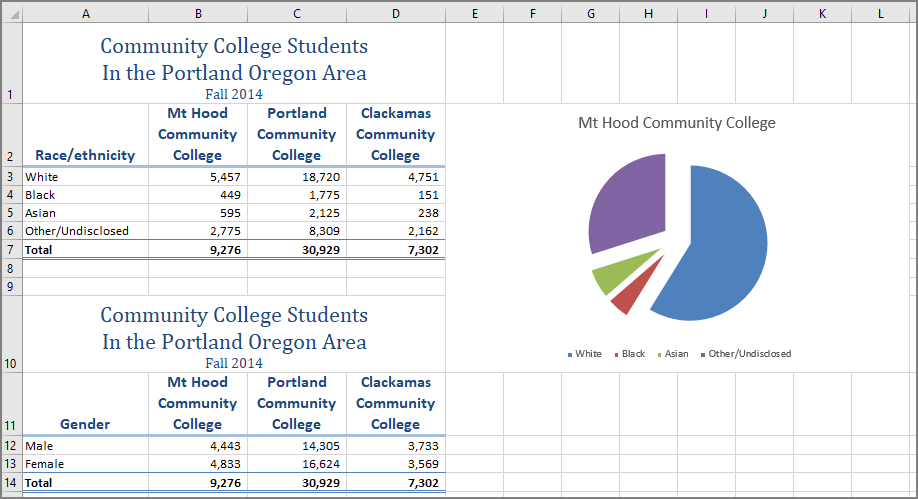
\includegraphics[width=\maxwidth{.95\linewidth}]{gfx/ch04_fig21}
			\caption{Pie Chart Moved and Resized}
			\label{04:fig21}
		\end{figure}
	
		\item Click the chart legend once and tap \fmtKeystroke{Delete}. A pie chart typically shows labels next to each slice, so the legend is unnecessary.
		\item Right-click any of the slices in the pie chart and select \fmtButton{Add Data Labels} from the list. This will add the values for each of the slices in the pie.
		\item Now, right-click one of the numbers that was just added to the pie chart and select \fmtButton{Format Data Labels} from the list. This will open the \textit{Format Data Labels} pane on the right.
		\item Check the boxes for \fmtButton{Category Name} and \fmtButton{Percentage} then uncheck the \fmtButton{Value} box in the \textit{Label Options} section in the \textit{Format Data Labels} pane (see Figure \ref{04:fig22}).
		\item Click the \fmtButton{Close} button at the top of the \textit{Format Data Labels} pane.
		\item Select the data labels again (if needed) by clicking on one of the labels. Click \fmtButton{Home $ \Rightarrow $ Font $ \Rightarrow $ Bold} to make the labels bold font.
		\item Save the \fmtWorksheet{CH4-Charting} workbook.
	\end{enumerate}
\end{enumbox}

\begin{figure}[H]
	\centering
	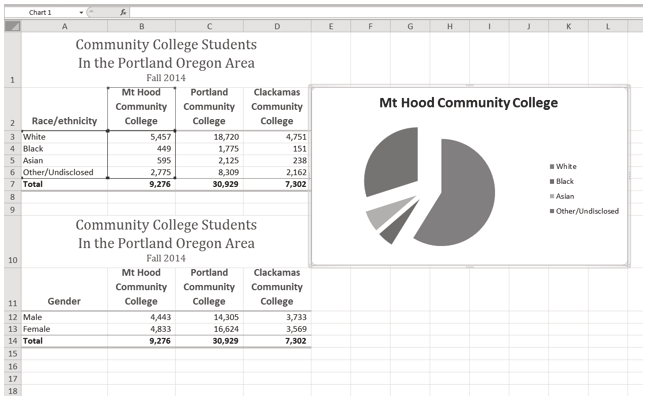
\includegraphics[width=\maxwidth{.95\linewidth}]{gfx/ch04_fig22}
	\caption{Final Settings in the Format Data Labels Pane}
	\label{04:fig22}
\end{figure}

Although there are no specific limits for the number of categories used on a pie chart, a good rule of thumb is ten or less. As the number of  categories exceeds ten, it becomes more challenging to identify key categories that comprise most of the total. Figure \ref{04:fig23} shows the completed pie chart.

\begin{figure}[H]
	\centering
	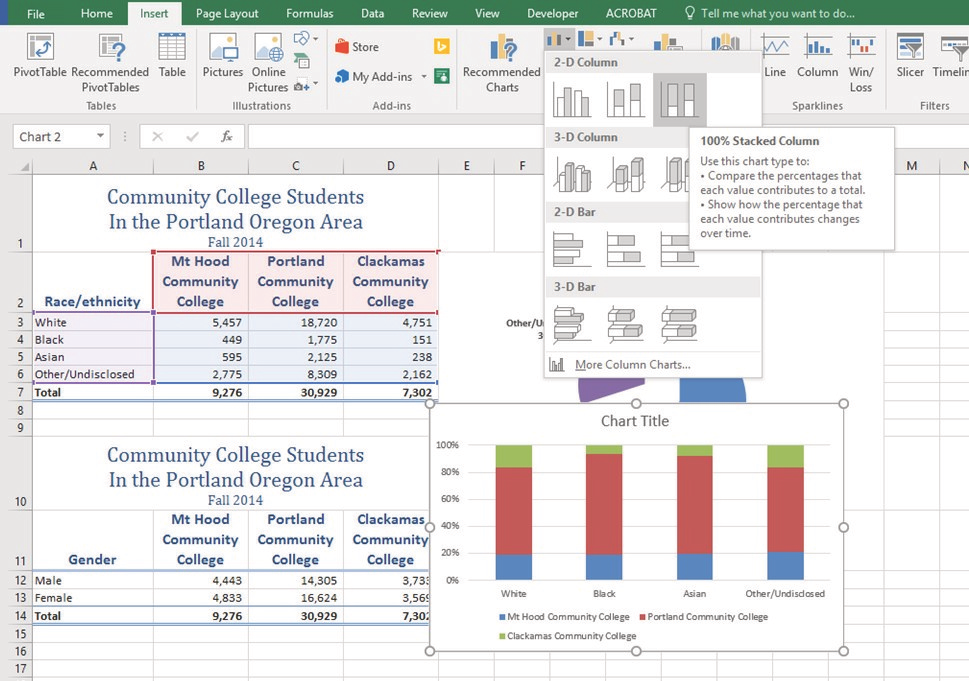
\includegraphics[width=\maxwidth{.95\linewidth}]{gfx/ch04_fig23}
	\caption{Final Enrollment Statistics Pie Chart}
	\label{04:fig23}
\end{figure}

\begin{center}
	\begin{sklbox}{Skill Refresher}
		\textbf{Inserting a Pie Chart}
		\\
		\begin{itemize}
			\setlength{\itemsep}{0pt}
			\setlength{\parskip}{0pt}
			\setlength{\parsep}{0pt}

			\item Select a range of cells that contain the data used to create the chart.
			\item Click \textit{Insert $ \Rightarrow $ Charts $ \Rightarrow $ Pie}.
			\item Select a format option from the Pie Chart drop-down menu.
			
		\end{itemize}
	\end{sklbox}
\end{center}

\subsection{Percent of Total: Stacked Column Chart}

The last chart type demonstrated in this chapter is the stacked column chart. A stacked column chart is used  to show a percent of a total. For example, the data on the \textit{Enrollment Statistics} worksheet shows student enrollment by race for several colleges. Suppose that it was necessary to show all the data for all colleges.

\begin{enumbox}
	\begin{enumerate}
		\item Click the \fmtWorksheet{Enrollment Statistics} worksheet to activate it if it is not already activated.
		\item Select \fmtLoc{A2:D6}.
		\item Click \fmtButton{Insert $ \Rightarrow $ Charts $ \Rightarrow $ Column}.	Select the \fmtButton{100\% Stacked Column} format option from 2-D Column section in the drop-down list (see Figure \ref{04:fig24}).
	\end{enumerate}
\end{enumbox}
	
\begin{figure}[H]
	\centering
	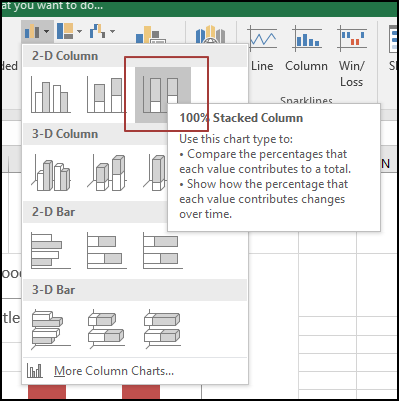
\includegraphics[width=\maxwidth{.65\linewidth}]{gfx/ch04_fig24}
	\caption{Selecting the 100\% Stacked Column Chart}
	\label{04:fig24}
\end{figure}

Figure \ref{04:fig25} shows the column chart created after selecting the \textit{100\% Stacked Column} format option. As mentioned, the goal of this chart is to show the enrollment of students by race. However, notice that Excel places the racial categories on the X-Axis. It would be more useful if the college names were on that axis instead.

\begin{figure}[H]
	\centering
	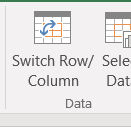
\includegraphics[width=\maxwidth{.95\linewidth}]{gfx/ch04_fig25}
	\caption{Initial Construction of the 100\% Stacked Column Chart}
	\label{04:fig25}
\end{figure}

Excel organized the data this way because there are more Race/ethnicity categories (data in \textit{Column A}) than colleges (data in \textit{Row 2}). This organization is not a wrong guess on Excel's part, but this is not what is wanted in this case. The following steps explain how to correct this problem and complete the chart.

\begin{enumbox}
	\begin{enumerate}
		\item Click \fmtButton{Chart Tools Design $ \Rightarrow $ Data $ \Rightarrow $ Switch Row/Column}. This option reverses the legend and current \textit{X-Y Axis} categories. (\fmtNewExcel{Excel 365} named the tab \textit{Chart Design}.)
	
		\begin{figure}[H]
			\centering
			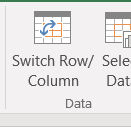
\includegraphics[width=\maxwidth{.95\linewidth}]{gfx/ch04_fig26}
			\caption{Switch Row/Column}
			\label{04:fig26}
		\end{figure}
	
		\item Click and drag the chart so the upper left corner is in the middle of cell \fmtLoc{E12}.
		\item Resize the chart using the following values. For each side of the chart, press and hold \fmtKeystroke{Alt}, then left-click and drag the resize handle on the chart to make it ``lock into'' position.
	
		\begin{table}[H]
		\rowcolors{1}{}{tablerow} % zebra striping background
		\captionsetup{labelformat=empty} % kill the label and caption area
		{\small
			%\fontsize{8}{10} \selectfont %Replace small for special font size
			\begin{longtable}{R{0.75in}L{1.50in}} %Left-aligned, Max width: 4.25in
				\textbf{Chart Side} & \textbf{Locked To} \endhead
				\hline
				Top & Top of \fmtLoc{Row 12}\\
				Left & Left of \fmtLoc{Column E}\\
				Bottom & Bottom of \fmtLoc{Row 30}\\
				Right & Right of \fmtLoc{Column N}\\
			\end{longtable}
		} % End small
		\end{table}
	
		\item Click the legend one time, then tap \fmtKeystroke{Delete}.
		\item Add a Data Table. This option is another way of displaying a legend for a column chart along with the numerical values that make up each component.
		\item Click \fmtButton{Chart Tools Design $ \Rightarrow $ Chart Layouts $ \Rightarrow $ Add Chart Element $ \Rightarrow $ Data Table $ \Rightarrow $ With Legend Keys}. (\fmtNewExcel{Excel 365} named the tab \textit{Chart Design}.)
		\item Change the Chart Title to \fmtTyping{Enrollment by Race}. If there is no chart title, click \fmtButton{Chart Tools Design $ \Rightarrow $ Chart Layouts $ \Rightarrow $ Add Chart Element $ \Rightarrow $ Chart Title $ \Rightarrow $ Above Chart}. (\fmtNewExcel{Excel 365} named the tab \textit{Chart Design}.)
		\item Save the \fmtWorksheet{CH4-Charting} workbook.
	\end{enumerate}
\end{enumbox}
	
Figure \ref{04:fig27} shows the final stacked column chart. Notice the similarities and differences in the enrollments at the local community colleges.

\begin{figure}[H]
	\centering
	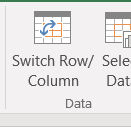
\includegraphics[width=\maxwidth{.95\linewidth}]{gfx/ch04_fig27}
	\caption{Final 100\% Stacked Column Chart}
	\label{04:fig27}
\end{figure}

\begin{center}
	\begin{sklbox}{Skill Refresher}
		\textbf{Inserting a Stacked Column Chart}
		\\
		\begin{itemize}
			\setlength{\itemsep}{0pt}
			\setlength{\parskip}{0pt}
			\setlength{\parsep}{0pt}

			\item Select a range of cells that contain data that will be used to create the chart.
			\item Click \textit{Insert $ \Rightarrow $ Charts $ \Rightarrow $ Column}.
			\item Select the \textit{Stacked Column} format option from the \textit{Column Chart} drop-down menu to show the values of each category on the Y-Axis. Select the \textit{100\% Stacked Column} option to show the percent of total for each category on the Y-Axis.
			
		\end{itemize}
	\end{sklbox}
\end{center}

\begin{center}
	\begin{tkwbox}{Key Take-Aways}
		\textbf{Save}
		\\
		\begin{itemize}
			\setlength{\itemsep}{0pt}
			\setlength{\parskip}{0pt}
			\setlength{\parsep}{0pt}
			
			\item Identifying the message to be conveyed to an audience is a critical first step in creating an Excel chart.
			\item Both a column chart and a line chart can be used to present a trend over a period. However, a line chart is preferred over a column chart when presenting data over long periods of time.
			\item The number of bars on a column chart should be limited to twenty bars or less.
			\item When creating a chart to compare trends, the values for each data series must be within a reasonable range. If there is a wide variance between the values in the two data series (two times or more), the percent change should be calculated with respect to the first data point for each series.
			\item When working with frequency distributions, the use of a column chart or a bar chart is a matter of preference. However, a column chart is preferred when working with a trend over a period.
			\item A pie chart is used to present the percent of total for a data set.
			\item A stacked column chart is used to show how a percent total changes over time.

		\end{itemize}
	\end{tkwbox}
\end{center}

\section{Formatting Charts}

\begin{center}
	\begin{objbox}{Learning Objectives}
		\begin{itemize}
			\setlength{\itemsep}{0pt}
			\setlength{\parskip}{0pt}
			\setlength{\parsep}{0pt}

			\item Apply formatting commands to the X-Axis and Y-Axis.
			\item Enhance the visual appearance of the chart title and chart legend by using various formatting techniques.
			\item Assign titles to the X-Axis and Y-Axis that clarify labels and numeric values for the reader.
			\item Apply labels and formatting techniques to the data series in the plot area of a chart.
			\item Apply formatting commands to the chart area and the plot area of a chart.
			\item Employ series lines and annotations to enhance trends and provide additional information on a chart.
			
		\end{itemize}
	\end{objbox}
\end{center}

Various formatting techniques can be used to enhance the appearance of a chart once it is created. Formatting commands are applied to a chart for the same reason they are applied to a worksheet; they make the chart easier to read. However, formatting techniques help qualify and explain the data in a chart. For example, footnotes that explain the data source or clarify the magnitude of truncated numbers can be added. These notes are also helpful in answering questions when using charts in a live presentation. This section demonstrates these formatting techniques using the previous section's column and stacked column chart.

\subsection{Axis Formats}

Numerous formatting commands can be applied to a chart's X-Axis and Y-Axis. Although adjusting the font size, style, and color are common; many more options are available through the \textit{Format Axis} pane. The following steps demonstrate some formatting techniques on the \textit{Grade Distribution Comparison} chart. (Note: this section continues the previous exercise. Students who only need to complete this section can open \fmtWorksheet{CH4-Charting Solution 1\_1} to start where the previous exercise ended.)

\begin{enumbox}
	\begin{enumerate}
		\item Switch to the \fmtWorksheet{Grade Distribution} worksheet and click anywhere along the X-Axis (horizontal axis) of the \textit{Grade Distribution Comparison} chart. 
		\item Right-click and select \fmtButton{Font}.
		\item Change the font to Arial, the Font Style to Bold, and the Size to $ 11 $ (see Figure \ref{04:fig28}).
		\item Click \fmtButton{OK}.
	
		\begin{figure}[H]
			\centering
			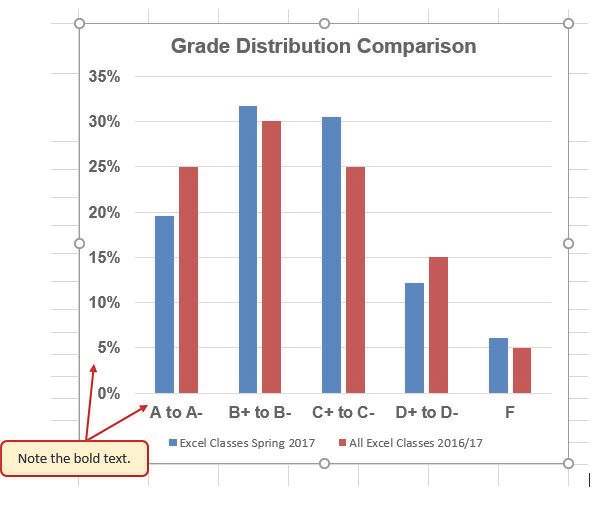
\includegraphics[width=\maxwidth{.95\linewidth}]{gfx/ch04_fig28}
			\caption{Font Dialog Box}
			\label{04:fig28}
		\end{figure}
	
		\item Click anywhere along the Y-Axis to activate it.
		\item Right-click and select \fmtButton{Font}.
		\item Change the font to Arial, the Font Style to Bold, and the Size to $ 11 $.
		\item Click on the chart title.
		\item Right-click and select \fmtButton{Font}.
		\item Change the font to Arial, the Font Style to Bold, and the Size to $ 14 $.
		\item The final appearance of the axes is shown in Figure \ref{04:fig29}.
	\end{enumerate}
\end{enumbox}
	
\begin{figure}[H]
	\centering
	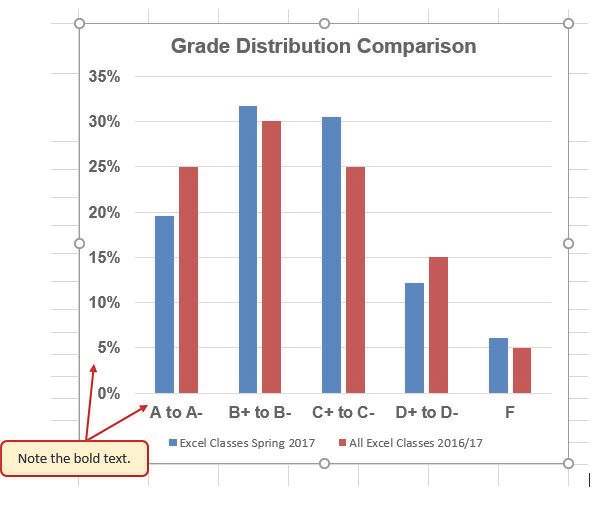
\includegraphics[width=\maxwidth{.95\linewidth}]{gfx/ch04_fig29}
	\caption{Formatted X and Y Axes}
	\label{04:fig29}
\end{figure}

Next, change the percentage numbers on the Y-Axis (vertical axis).

\begin{enumbox}
	\begin{enumerate}
		\item Right-click the Y-Axis. 
		\item Select \fmtButton{Format Axis}. This opens the \textit{Format Axis} pane.
		\item Click \fmtButton{Number} at the bottom of list of options. The options in this section of the \textit{Format Axis} pane are used to format the numbers that appear on the axis.
		\item Click in the \textit{Decimal} places input box and change the value to $ 1 $.
		\item Select \fmtButton{Axis Options} at the top of the list of options. 
		\item Change the \textit{Minimum Bound} to $ .05 $ to make the differences in the columns more dramatic. The \textit{Format Axis} pane should match Figure \ref{04:fig30}.
		\item Click the \fmtButton{Close} button at the top of the \textit{Format Axis} pane.
		\item Save the \fmtWorksheet{CH4-Charting} workbook.
	\end{enumerate}
\end{enumbox}
	
\begin{figure}[H]
	\centering
	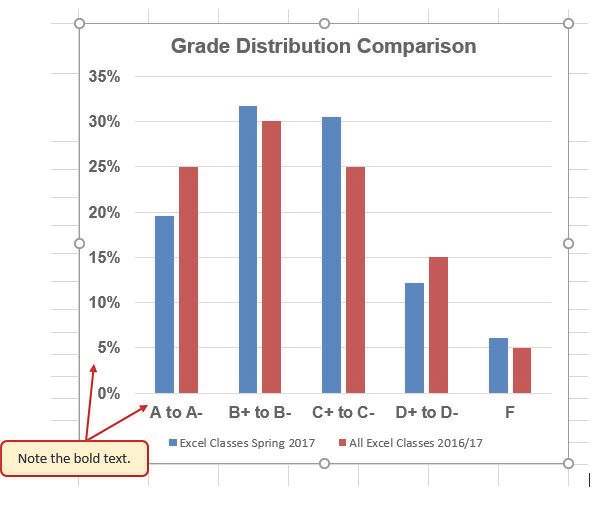
\includegraphics[width=\maxwidth{.95\linewidth}]{gfx/ch04_fig30}
	\caption{Format Axis Pane Changes}
	\label{04:fig30}
\end{figure}

\begin{center}
	\begin{infobox}{Note}
		\textbf{Experiment!}
		\\
		\\
		The font styling can also be changed using shortcut keys and the buttons on the \textit{Home} tab.
	\end{infobox}
\end{center}

\begin{center}
	\begin{sklbox}{Skill Refresher}
		\textbf{Formatting the X-Axis and Y-Axis}
		\\
		\begin{itemize}
			\setlength{\itemsep}{0pt}
			\setlength{\parskip}{0pt}
			\setlength{\parsep}{0pt}

			\item Click anywhere along the X-Axis or Y-Axis to activate it.
			\item Click either the \textit{Home} tab or \textit{Chart Tools Design} tab of the ribbon.
			\item Select any of the available formatting commands in these tabs.
			
		\end{itemize}
	\end{sklbox}
\end{center}

\begin{center}
	\begin{sklbox}{Skill Refresher}
		\textbf{X-Axis and Y-Axis Number Formats}
		\\
		\begin{itemize}
			\setlength{\itemsep}{0pt}
			\setlength{\parskip}{0pt}
			\setlength{\parsep}{0pt}

			\item Click anywhere along the X-Axis or Y-Axis to activate it.
			\item Click \textit{Chart Tools Format $ \Rightarrow $ Format Selection}.
			\item Click \textit{Number} from the list of options on the left side of the \textit{Format Axis} dialog box.
			\item Select a number format and set decimal places on the right side of the \textit{Format Axis} dialog box.
			\item Click the \textit{Close} button in the \textit{Format Axis} pane.
			
		\end{itemize}
	\end{sklbox}
\end{center}

\subsection{Chart Legend and Title Formats}

The chart legend and title should be formatted next. Like the X-Axis and the Y-Axis, format these items by activating them and using commands in the \textit{Home} tab or the \textit{Format} pane. The following steps explain how to change these formats.

\begin{enumbox}
	\begin{enumerate}
		\item Right-click the legend on the \textit{Grade Distribution Comparison} chart and select \fmtButton{Format Legend}.
		\item Select \fmtButton{Right} in the \textit{Legend Position} options. 
		\item Close the \textit{Format Legend} pane.
		\item Move the legend by placing the cursor, shaped like a plus sign with four arrows, on the edge of the selection box. Click and drag the legend so the top of the legend aligns with the $ 35\% $ line next to the plot area (see Figure \ref{04:fig31}).
	
		\begin{figure}[H]
			\centering
			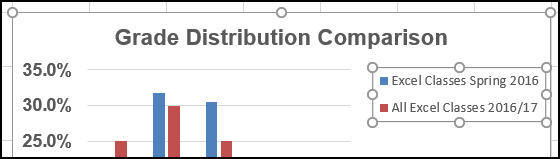
\includegraphics[width=\maxwidth{.95\linewidth}]{gfx/ch04_fig31}
			\caption{Moving the Legend}
			\label{04:fig31}
		\end{figure}
	
		\item While the legend is still selected, change \fmtButton{Home $ \Rightarrow $ Font} to Arial, Bold, Italics, Size $ 12 $.
		\item Click and drag the left sizing handle, so the legend is just touching the horizontal grid lines of the plot area and the bottom sizing handle, so the entire legend is visible (see Figure \ref{04:fig32}).
	
		\begin{figure}[H]
			\centering
			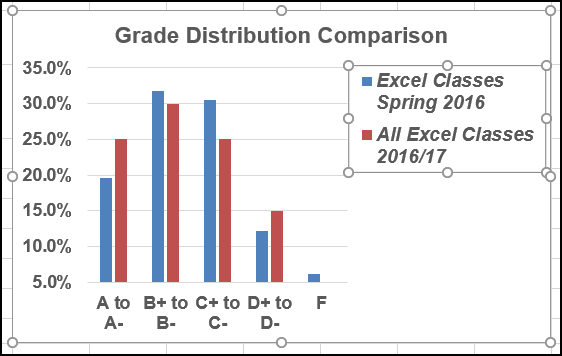
\includegraphics[width=\maxwidth{.95\linewidth}]{gfx/ch04_fig32}
			\caption{Legend Formatted and Resized}
			\label{04:fig32}
		\end{figure}
	
		\item Right-click on the chart title and select \fmtButton{Format Chart Title} to open the \textit{Format Chart Title} pane (see Figure \ref{04:fig33}).
		\item Under \textit{Title Options} in the Effects group (the option in the middle), select the first \textit{outer} preset shadow. 
		\item Select \textit{Blue, Accent 1} as the shadow color.
		\item Close the \textit{Format Chart Title} pane.
		\item Save the \fmtWorksheet{CH4-Charting} workbook.
	\end{enumerate}
\end{enumbox}
	
\begin{figure}[H]
	\centering
	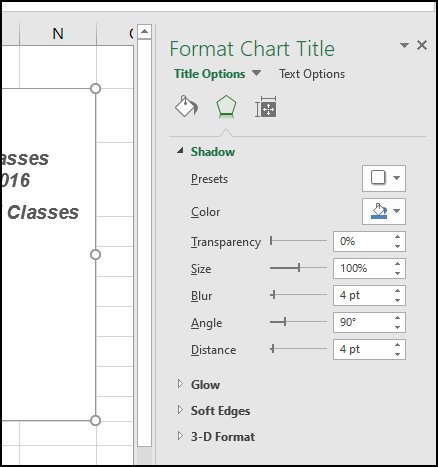
\includegraphics[width=\maxwidth{.75\linewidth}]{gfx/ch04_fig33}
	\caption{Format Chart Title Pane}
	\label{04:fig33}
\end{figure}

\begin{center}
	\begin{sklbox}{Skill Refresher}
		\textbf{Formatting the Chart Legend}
		\\
		\begin{itemize}
			\setlength{\itemsep}{0pt}
			\setlength{\parskip}{0pt}
			\setlength{\parsep}{0pt}

			\item Click the Legend to activate it.
			\item Click either the \textit{Home} tab or right-click to activate the appropriate formatting pane.
			\item Select any of the available formatting commands.
			\item Click and drag the legend to move it.
			\item Click and drag any of the sizing handles to adjust the size of the legend.
			
		\end{itemize}
	\end{sklbox}
\end{center}

\begin{center}
	\begin{sklbox}{Skill Refresher}
		\textbf{Formatting the Chart Title}
		\\
		\begin{itemize}
			\setlength{\itemsep}{0pt}
			\setlength{\parskip}{0pt}
			\setlength{\parsep}{0pt}

			\item Click anywhere on the chart title.
			\item Click either the \textit{Home} tab or right-click to activate the appropriate formatting pane.
			\item Select any of the available formatting commands.
			
		\end{itemize}
	\end{sklbox}
\end{center}

\subsection{X-Axis and Y-Axis Titles}

Titles for the X-Axis and Y-Axis are necessary for defining the numbers and categories presented on a chart. For example, looking at the \textit{Grade Distribution Comparison} chart, it is unclear what the percentages along the Y-Axis represent. The following steps explain how to add titles to the X-Axis and Y-Axis to define these numbers and categories.

\begin{enumbox}
	\begin{enumerate}
		\item Click anywhere on the \textit{Grade Distribution Comparison} chart in the \fmtWorksheet{Grade Distribution} worksheet to activate it.
		\item Click \fmtButton{Chart Tools Design $ \Rightarrow $ Chart Layouts $ \Rightarrow $ Add Chart Element $ \Rightarrow $ Axis Titles $ \Rightarrow $ Primary Vertical} (See Figure \ref{04:fig34}). (\fmtNewExcel{Excel 365} named the tab \textit{Chart Design}.)
	
		\begin{figure}[H]
			\centering
			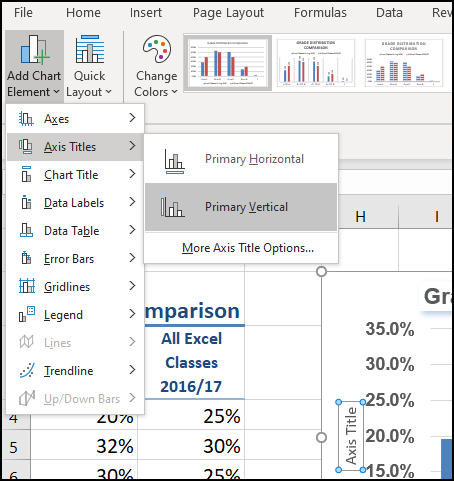
\includegraphics[width=\maxwidth{.95\linewidth}]{gfx/ch04_fig34}
			\caption{Adding a Title for the Y-Axis}
			\label{04:fig34}
		\end{figure}
	
		\item Using \fmtButton{Home $ \Rightarrow $ Font}, change the font of the axis title to Arial, Bold, Size $ 11 $.
		\item Click in the beginning of the Y-Axis title and delete the generic title, then type \fmtTyping{Percent of Enrolled Students} (see Figure \ref{04:fig35}).
	\end{enumerate}
\end{enumbox}
	
\begin{figure}[H]
	\centering
	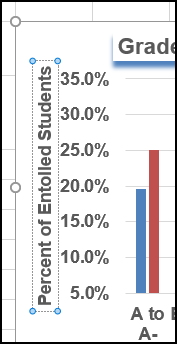
\includegraphics[width=\maxwidth{.95\linewidth}]{gfx/ch04_fig35}
	\caption{Adding and Formatting the Y-Axis Title}
	\label{04:fig35}
\end{figure}

Next, add the title for the X-Axis.

\begin{enumbox}
	\begin{enumerate}
		\item Click \fmtButton{Chart Tools Design $ \Rightarrow $ Chart Layouts $ \Rightarrow $ Add Chart Element $ \Rightarrow $ Axis Titles $ \Rightarrow $ Primary Horizontal}. (\fmtNewExcel{Excel 365} named the tab \textit{Chart Design}.)
		\item Using \fmtButton{Home $ \Rightarrow $ Font}, change the font of the axis title to Arial, Bold, Size $ 11 $. 
		\item Click in the beginning of the X-Axis title and delete the generic title, then type \fmtTyping{Final Course Grade}. Figure \ref{04:fig36} shows the added titles for the X-Axis and Y-Axis. The titles provide definitions for the grade categories along the X-Axis as well as the percentages on the Y-Axis.
		\item Save the \fmtWorksheet{CH4-Charting} workbook.
	\end{enumerate}
\end{enumbox}
	
\begin{figure}[H]
	\centering
	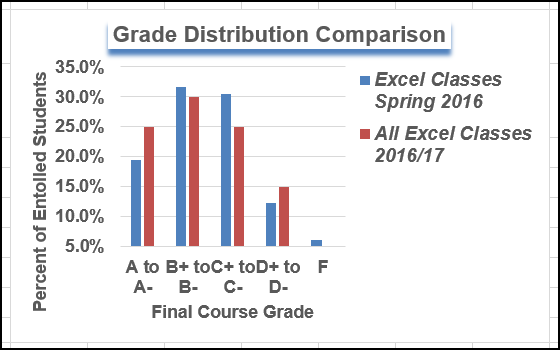
\includegraphics[width=\maxwidth{.95\linewidth}]{gfx/ch04_fig36}
	\caption{Axes Titles Added}
	\label{04:fig36}
\end{figure}

\begin{center}
	\begin{sklbox}{Skill Refresher}
		\textbf{X-Axis and Y-Axis Titles}
		\\
		\begin{itemize}
			\setlength{\itemsep}{0pt}
			\setlength{\parskip}{0pt}
			\setlength{\parsep}{0pt}

			\item Click anywhere on the chart to activate it.
			\item Click \textit{Chart Tools Design $ \Rightarrow $ Chart Layouts $ \Rightarrow $ Add Chart Element}.
			\item Select one of the options from the second drop-down list.
			\item Click in the axis title to remove the generic title and type a new title.
			
		\end{itemize}
	\end{sklbox}
\end{center}

\subsection{Data Series Labels and Formats}

A data series is an item displayed graphically on a chart; labeling it is a crucial formatting feature. For example, the blue bars on the \textit{Grade Distribution Comparison} chart represent one data series. Labels can be added at the end of each bar to show the exact percentage the bar represents. In addition, other formatting enhancements can be added to the data series, such as changing the color of the bars or adding an effect. The following steps explain adding these labels and formats to the chart.

\begin{enumbox}
	\begin{enumerate}
		\item Click on any of the red bars representing the \textit{All Excel Classes} data series on the \textit{Grade Distribution Comparison} chart in the \fmtWorksheet{Grade Distribution} worksheet. Clicking one bar automatically activates all bars in the data series. If a bar is clicked a second time, only that one bar is activated.
		\item Right-click and select \fmtButton{Format Data Series} to open the \textit{Format Data Series} pane.
		\item Click the \fmtButton{Fill and Line} (paint bucket) button to bring up the \textit{Fill and Border} group of commands.
		\item Click the word \fmtButton{Fill} (if needed) to expand the list of Fill options.
		\item Select \fmtButton{Pattern Fill}. Then select \textit{Dotted: }$ 30\% $ (fifth column, top row). Changing the fill pattern to a pattern makes it easier to distinguish between the data series when the chart is printed or viewed in black and white. Experiment with the fill pattern by selecting different foreground and background colors.
		\item Close the \textit{Format Data Series} pane.
	\end{enumerate}
\end{enumbox}
	
\begin{figure}[H]
	\centering
	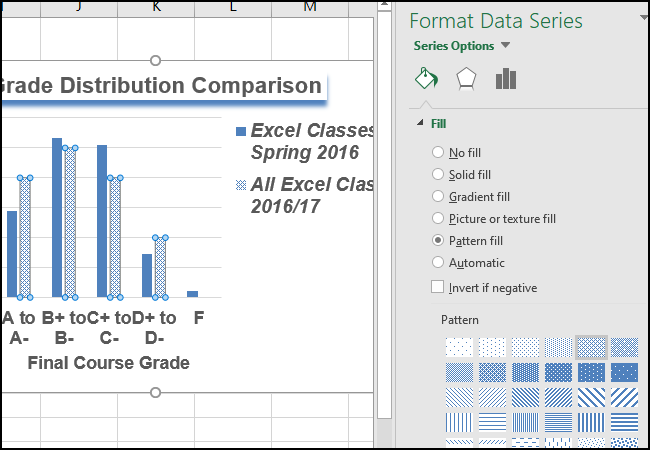
\includegraphics[width=\maxwidth{.95\linewidth}]{gfx/ch04_fig37}
	\caption{Changing the Fill of a Data Series}
	\label{04:fig37}
\end{figure}

Next, add the Data Labels at the end of the columns.

\begin{enumbox}
	\begin{enumerate}
		\item Be sure that the entire chart is selected, not just one of the data series. 
		\item Click \fmtButton{Chart Tools Design $ \Rightarrow $ Chart Layouts $ \Rightarrow $ Add Chart Element $ \Rightarrow $ Data Labels $ \Rightarrow $ Outside End} (see Figure \ref{04:fig38}.) (\fmtNewExcel{Excel 365} named the tab \textit{Chart Design}.)
		\item Click on one of the Data Labels for the first data series. Notice that all the data labels for that data series are selected.
		\item Using \fmtButton{Home $ \Rightarrow $ Font}, change the font to Arial, Bold, Size $ 9 $.
		\item Click on one of the data labels for the second data series. Using \fmtButton{Home $ \Rightarrow $ Font}, change the font to Arial, Bold, Size $ 9 $.
		\item Save the \fmtWorksheet{CH4-Charting} workbook.
	\end{enumerate}
\end{enumbox}
	
\begin{figure}[H]
	\centering
	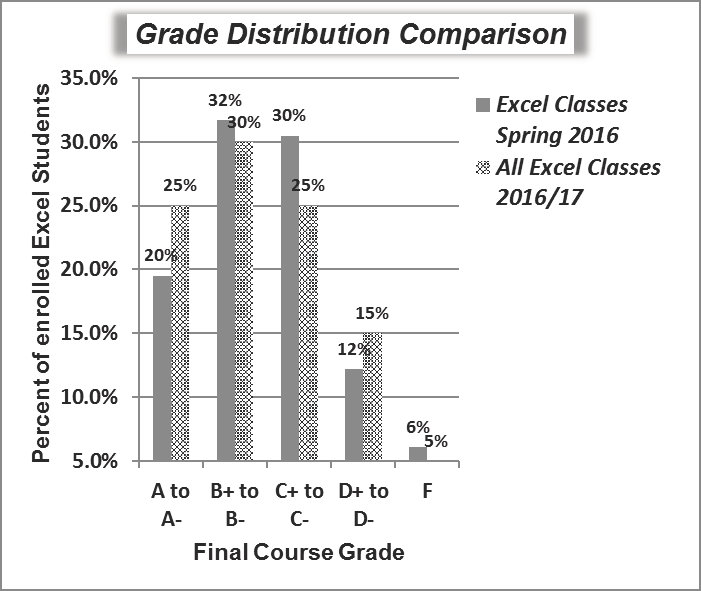
\includegraphics[width=\maxwidth{.75\linewidth}]{gfx/ch04_fig38}
	\caption{Adding Labels to a Data Series}
	\label{04:fig38}
\end{figure}

Figure \ref{04:fig39} shows the \textit{Grade Distribution Comparison} chart with the completed formatting adjustments and labels added to the data series. Note that each data label can be moved if two data labels overlap or if a data label falls in the middle of a grid line. To move an individual data label, click it twice and then click and drag.

\begin{figure}[H]
	\centering
	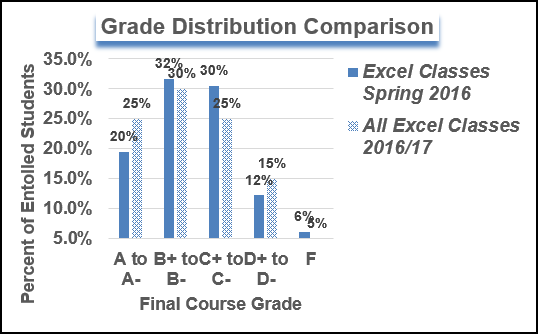
\includegraphics[width=\maxwidth{.95\linewidth}]{gfx/ch04_fig39}
	\caption{Completed Formatting Adjustments for the Data Series}
	\label{04:fig39}
\end{figure}

\begin{center}
	\begin{sklbox}{Skill Refresher}
		\textbf{Adding Data Labels}
		\\
		\begin{itemize}
			\setlength{\itemsep}{0pt}
			\setlength{\parskip}{0pt}
			\setlength{\parsep}{0pt}

			\item Click anywhere on the chart to activate it.
			\item Click \textit{Chart Tools Design $ \Rightarrow $ Chart Layouts $ \Rightarrow $ Add Chart Element}.
			\item Select \textit{Data Labels}
			\item Select one of the preset positions from the drop-down list.
			
		\end{itemize}
	\end{sklbox}
\end{center}

\begin{center}
	\begin{sklbox}{Skill Refresher}
		\textbf{Formatting a Data Series}
		\\
		\begin{itemize}
			\setlength{\itemsep}{0pt}
			\setlength{\parskip}{0pt}
			\setlength{\parsep}{0pt}
			
			\item Click any bar or line for a data series.
			\item Right-click to activate the \textit{Format Data Series} pane.
			\item Use the formatting tools in the pane to make changes to the data series.
			
		\end{itemize}
	\end{sklbox}
\end{center}

\subsection{Adding Series Lines and Annotations to a Chart}

Series lines are used in stacked column charts to show the change from one stack to the next. Annotations help clarify the data presented in a chart or identify data sources. In addition to demonstrating these skills, this section will review several formatting skills covered earlier. 

\begin{enumbox}
	\begin{enumerate}
		\item Locate the \textit{Enrollment by Race} stacked column chart on the \fmtWorksheet{Enrollment Statistics} worksheet. Activate the chart by clicking anywhere inside the chart perimeter.
		\item Click \fmtButton{Chart Tools $ \Rightarrow $ Design $ \Rightarrow $ Location $ \Rightarrow $ Move Chart}. (\fmtNewExcel{Excel 365} named this tab \textit{Chart Design}.) 
		\item Select \textit{New sheet} and type the following in the input box: \fmtTyping{Enrollment by Race Chart}. 
		\item Click \fmtButton{OK}. The chart will be moved to a new worksheet, and that sheet will be activated.
		\item Click on the data table (on the X-Axis) to activate it. When active, the data table will have a resizing handle at each of the four corners.
		\item Using \fmtButton{Home $ \Rightarrow $ Font}, change the font to Arial, Bold, size $ 12 $.
		\item Click on the Y-Axis and apply the same formatting adjustments used in the data table. 
		\item Click \fmtButton{Chart Tools Design $ \Rightarrow $ Chart Layouts $ \Rightarrow $ Add Chart Element $ \Rightarrow $ Axis Titles $ \Rightarrow $ Primary Vertical}. (\fmtNewExcel{Excel 365} named the tab \textit{Chart Design}.)
		\item Double-click in the default Y-Axis title and change it to \fmtTyping{Percent Enrollment by Race}.
		\item Click the border of the Y-Axis title to select the full title. The title will have a resizing handle at each of the four corners when active.
		\item Using \fmtButton{Home $ \Rightarrow $ Font}, change the font to Arial, Bold, size $ 14 $.
		\item Click \fmtButton{Chart Tools Design $ \Rightarrow $ Chart Layouts $ \Rightarrow $ Add Chart Element $ \Rightarrow $ Axis Titles $ \Rightarrow $ More Axis Title Options}. (\fmtNewExcel{Excel 365} named the tab \textit{Chart Design}.)
		\item Click the Y-Axis title to select it. The title will have a resizing handle at each of the four corners when active.
		\item In the \textit{Format Axis Title} pane, change the fill color to \textit{Blue, Accent 1, Lighter 80\%}, and the border color to \textit{Dark Blue, Text 2, Lighter 60\%} .
		\item Check the horizontal axis to see if this process created an extra axis title. If it did, delete it.
		\item Activate the title of the chart by clicking it once. The \textit{Format Chart Title} pane should be open. If not, right-click the Chart title and select \fmtButton{Format Chart Title} from the menu. Change the fill and border to match the vertical Axis label.
		\item Using \fmtButton{Home $ \Rightarrow $ Font}, change the chart title font to Arial, Bold, size $ 20 $.
		\item Close the \textit{Format Chart Title} pane.
		\item Click \fmtButton{Chart Tools Design $ \Rightarrow $ Chart Layouts $ \Rightarrow $ Add Chart Elements $ \Rightarrow $ Lines $ \Rightarrow $ Series Lines}. (\fmtNewExcel{Excel 365} named the tab \textit{Chart Design}.) This option adds lines to the chart, connecting each data series between the three stacks (see Figure \ref{04:fig40}).
	
		\begin{figure}[H]
			\centering
			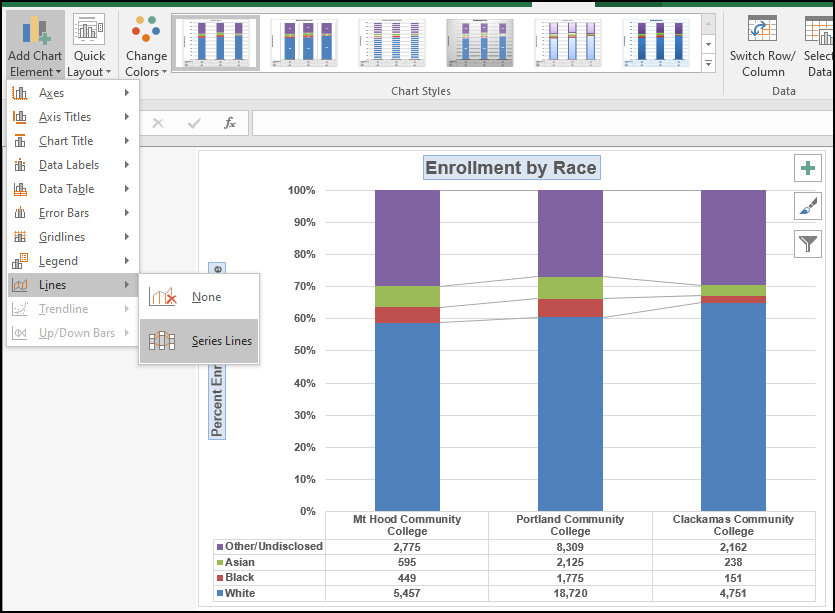
\includegraphics[width=\maxwidth{.95\linewidth}]{gfx/ch04_fig40}
			\caption{Selecting the Series Lines Option}
			\label{04:fig40}
		\end{figure}

		\item Right-click on any of the series lines added to the chart. Clicking one line will activate all lines on the chart. (If the \textit{Format} pane is open, there is no need to right-click. Just left-click on any series line to change the formatting pane to \textit{Format Series Lines}.)
		\item Select \fmtButton{Format Series Lines} to open the \textit{Format Series Lines} pane.
		\item Change the width to $ 2.25 $ pt.
		\item Close the \textit{Format Series Lines} pane.
	\end{enumerate}
\end{enumbox}

Figure \ref{04:fig41} shows the chart's appearance with lines connecting the two stacks. This formatting enhancement is common for stacked column charts. The lines help focus the audience's attention on changes in the percent of the total.

\begin{figure}[H]
	\centering
	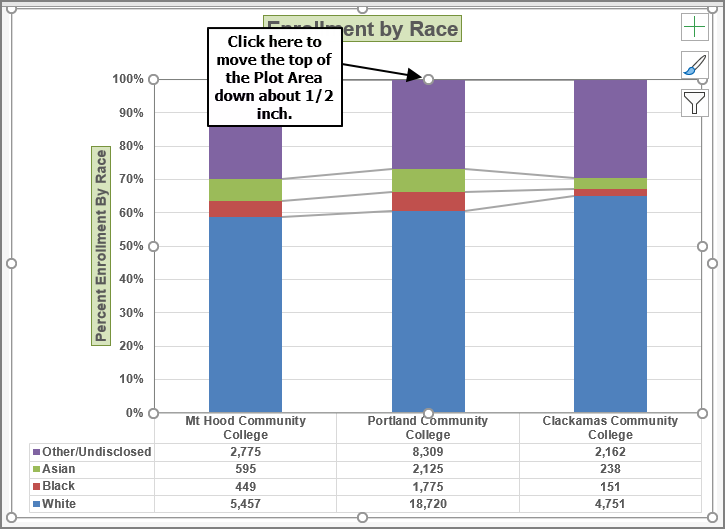
\includegraphics[width=\maxwidth{.95\linewidth}]{gfx/ch04_fig41}
	\caption{Series Lines Added to the Stacked Column Chart}
	\label{04:fig41}
\end{figure}

The chart demonstrates the percentage differences in enrollment between the community colleges. However, it would be handy to know the total enrollment at each college. To display that, add text boxes above each column. To start, make room for the text boxes.

\begin{enumbox}
	\begin{enumerate}
		\item Select the Plot Area. Place cursor on the top center handle of the Plot Area and drag down about $ 1/2 $ inch. (See Figure \ref{04:fig42}.)
	\end{enumerate}
\end{enumbox}
	
\begin{figure}[H]
	\centering
	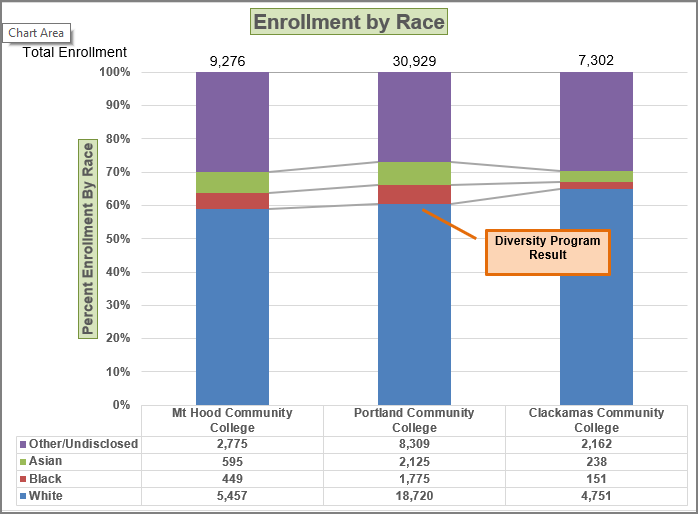
\includegraphics[width=\maxwidth{.95\linewidth}]{gfx/ch04_fig42}
	\caption{Resizing the Plot Area}
	\label{04:fig42}
\end{figure}

\subsection{Add Additional Information to the Chart.}

\begin{enumbox}
	\begin{enumerate}
		\item Click \fmtButton{Insert $ \Rightarrow $ Text $ \Rightarrow $ Text Box}.
		\item Place the mouse pointer on the left edge of the chart area approximately one-quarter inch from the top. Click and drag a rectangle approximately one and a half inches wide and one-quarter inch high. Do not worry if it is not exact, it will be moved and resized later.
		\item Type \fmtTyping{Total Enrollment} in the text box.
		\item Select all the text in the text box. (The text can be selected by either dragging over it with the mouse or by clicking on the border of the text box once). 
		\item Click \fmtButton{Home $ \Rightarrow $ Font}. Change the font to Arial, size $ 14 $.
		\item Resize and position the text box, so it fits above the $ 100\% $ label on the Y-Axis, as in \ref{04:fig43}
		\item Repeat the process to add and format text boxes above each column. The boxes can be copy/pasted to save time.
		\item In each text box, type the Total Enrollment for each school:
	
		\begin{itemize}
			\item Mt Hood --- 9,276
			\item Portland --- 30,929
			\item Clackamas --- 7,302
		\end{itemize}
		\item Check to be sure the text boxes look like Figure \ref{04:fig43} and then save the \fmtWorksheet{CH4-Charting} workbook.
	
		\begin{figure}[H]
			\centering
			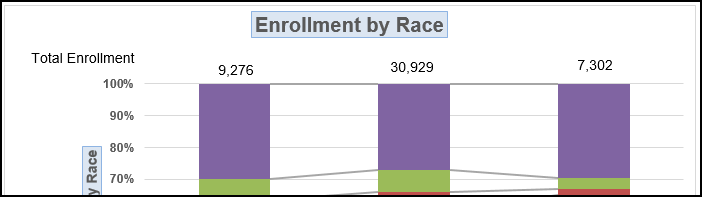
\includegraphics[width=\maxwidth{.95\linewidth}]{gfx/ch04_fig43}
			\caption{Enrollment Text boxes Added}
			\label{04:fig43}
		\end{figure}
	
		\item Excel also makes several graphic objects like circles, arrows, and stars available to draw attention to elements on charts. It is important to keep in mind the purpose of a chart is to present information to the audience, not show off the skill of the designer, so do not overdo these types of graphic objects.
		\item Click the chart to activate it if it is not already active.
		\item Click \fmtButton{Insert $ \Rightarrow $ Illustrations $ \Rightarrow $ Shapes $ \Rightarrow $ Callouts $ \Rightarrow $ Rounded Rectangular Callout} (see Figure \ref{04:fig44}). (\fmtNewExcel{Excel 365} named this callout \textit{Speech Bubble: Rectangle with Corners Rounded}.)
	
		\begin{figure}[H]
			\centering
			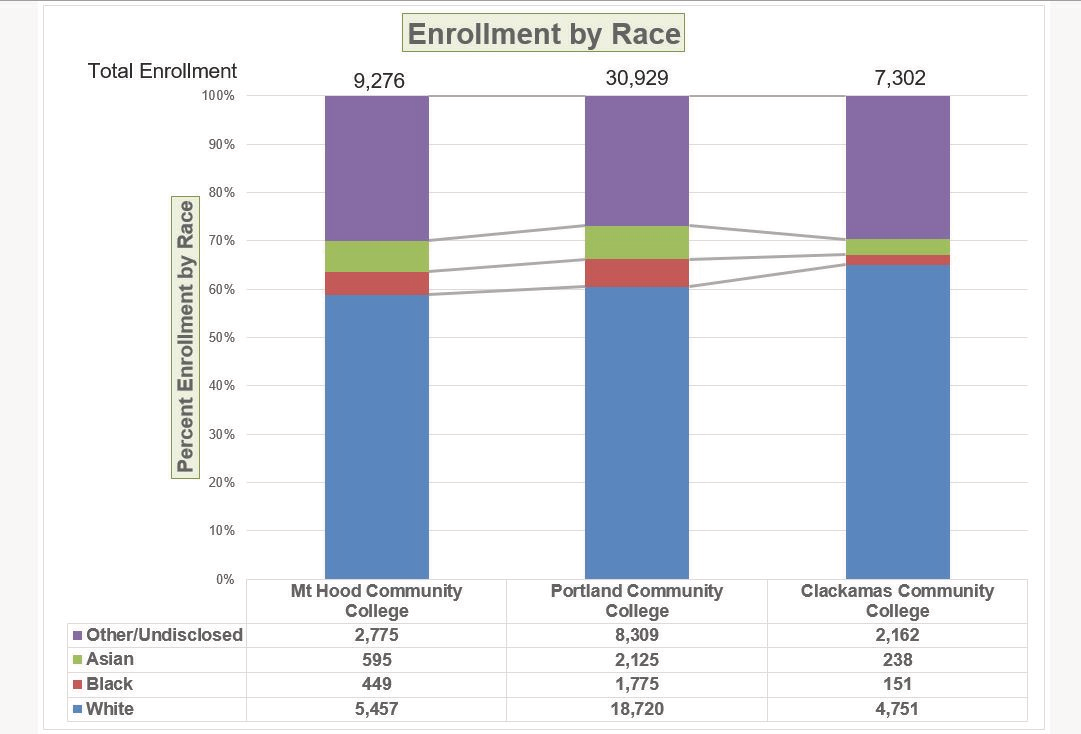
\includegraphics[width=\maxwidth{.45\linewidth}]{gfx/ch04_fig44}
			\caption{Selecting Rounded Rectangular Callout}
			\label{04:fig44}
		\end{figure}
	
		\item Drag a square on the graph. Do not worry about exact placement since the text square and callout line will be resized and repositioned later. See Figure \ref{04:fig45} for guidance.
		\item The callout is initially filled with blue, but that does not offer enough contrast with the chart bar. The \textit{Format Shape} panel opens when the callout is added. If the \textit{Format Shape} panel did not open, right-click on the callout and select \textit{Format Object}. Click the \textit{Shape Options} tab on the format panel and make these adjustments.
		
		\begin{enumerate}
			\item Select \textit{Orange, Accent 6, Lighter 60\%} as the fill color for the box.
			\item Select \textit{Orange, Accent 6, Darker 25\%} as the color for the line.
		\end{enumerate}
		
		\item Double-click inside the callout box and enter \fmtTyping{Diversity Program Result}.
		\item Click the border of the callout box to select it.
		\item Using \fmtButton{Home $ \Rightarrow $ Font}, change the font to Arial, $ 12 $pt, Bold font. 
		\item Click \fmtButton{Home $ \Rightarrow $ Alignment $ \Rightarrow $ Center}.
		\item Using the drag handles, resize and position the callout box so it is like Figure \ref{04:fig45}.
		\item Save the \fmtWorksheet{CH4-Charting} workbook.
	\end{enumerate}
\end{enumbox}
	
\begin{figure}[H]
	\centering
	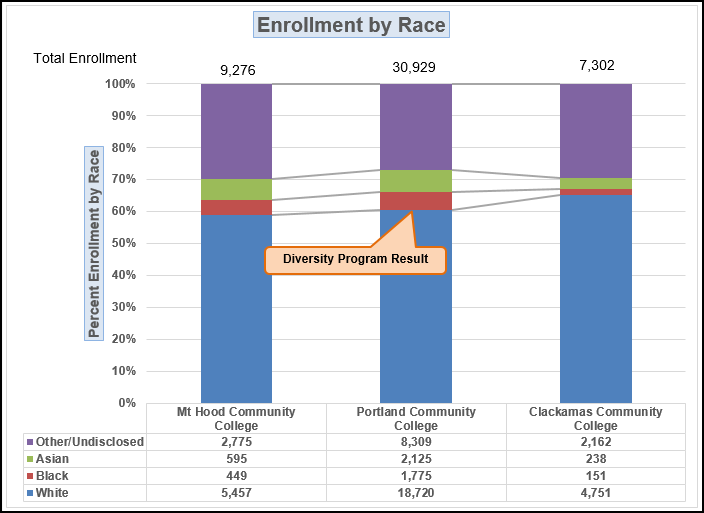
\includegraphics[width=\maxwidth{.95\linewidth}]{gfx/ch04_fig45}
	\caption{Completed Stacked Column Chart}
	\label{04:fig45}
\end{figure}

\begin{center}
	\begin{sklbox}{Skill Refresher}
		\textbf{Adding Series Lines}
		\\
		\begin{itemize}
			\setlength{\itemsep}{0pt}
			\setlength{\parskip}{0pt}
			\setlength{\parsep}{0pt}
			
			\item Click anywhere on the chart area.
			\item Click \textit{Chart Tools Design $ \Rightarrow $ Chart Layouts $ \Rightarrow $ Add Chart Elements $ \Rightarrow $ Lines $ \Rightarrow $ Series Lines}.
		\end{itemize}
	\end{sklbox}
\end{center}

\begin{center}
	\begin{sklbox}{Skill Refresher}
		\textbf{Adding Annotations}
		\\
		\begin{itemize}
			\setlength{\itemsep}{0pt}
			\setlength{\parskip}{0pt}
			\setlength{\parsep}{0pt}
			
			\item Click anywhere on the chart area.
			\item Click \textit{Insert $ \Rightarrow $ Text $ \Rightarrow $ Text Box}.
			\item Click and drag the size of the text box needed on the chart.
			\item Apply any desired format changes from the Home tab of the ribbon.
			\item Type the desired text.
			
		\end{itemize}
	\end{sklbox}
\end{center}

\begin{center}
	\begin{infobox}{Integrity Check}
		\textbf{Annotations and Axis Titles}
		\\
		\\
		Although adding annotations and axis titles can be a tedious process, doing so creates a high level of integrity for charts. People can misinterpret the message being conveyed by the chart if they make inaccurate assumptions about the values displayed. Axis titles and annotations help prevent readers from making false assumptions and ensure that readers see the most accurate representation of the message being conveyed by the chart.		
	\end{infobox}
\end{center}

\begin{center}
	\begin{tkwbox}{Key Take-Aways}
		\textbf{Formatting Charts}
		\\
		\begin{itemize}
			\setlength{\itemsep}{0pt}
			\setlength{\parskip}{0pt}
			\setlength{\parsep}{0pt}

			\item Applying appropriate formatting techniques is critical for making a chart easier to read.
			\item Many formatting commands in the \textit{Home} tab of the ribbon can be applied to a chart.
			\item To change the number format for a data label, use the \textit{Number} section in the \textit{Format Data Labels} dialog box. Note that number format commands in the \textit{Home} tab of the ribbon cannot be used for a data label.
			\item To change the number format for the values on the Y-Axis, and the X-Axis, use the \textit{Number} section of the \textit{Format Axis} dialog box. Note that number format commands in the \textit{Home} tab of the ribbon cannot be used for axis labels.
			\item Axis titles and annotations help prevent false assumptions from being made and ensure that the reader sees the most accurate representation of the information presented on a chart.
			
		\end{itemize}
	\end{tkwbox}
\end{center}

\section{Using Charts with Microsoft Word and Microsoft PowerPoint}

\begin{center}
	\begin{objbox}{Learning Objectives}
		\begin{itemize}
			\setlength{\itemsep}{0pt}
			\setlength{\parskip}{0pt}
			\setlength{\parsep}{0pt}

			\item Learn how to paste an image of an Excel chart into a Word document.
			\item Learn how to paste a link to an Excel chart into a PowerPoint slide.
			
		\end{itemize}
	\end{objbox}
\end{center}

Charts created in Excel are used in Microsoft Word documents or PowerPoint presentations, and Excel provides options for pasting a chart's image into either. Additionally, a link between Excel and Word or PowerPoint can be established so that if the data changes in the Excel file, it is automatically updated in the Word or PowerPoint files. Both methods of sharing a chart are covered in this section.

\subsection{Pasting a Chart Image Into Word}

This exercise needs two files:

\begin{itemize}
	\item The Excel spreadsheet used in this chapter: \textit{CH4-Charting}. (Note: this section continues the previous exercise. Students who only need to complete this section can open \textit{CH4-Charting Solution 1\_2} to start where the previous exercise ended.)
	\item This Word document: \textit{CH4-Diversity}
\end{itemize}

Excel charts can be valuable tools for explaining quantitative data in a written report. Reports that address business plans, public policies, and budgets, to name a few, involve quantitative data. For this example, assume that the \textit{Enrollment by Race} stacked column chart (Figure \ref{04:fig45}) is used in a student's written report. The following steps demonstrate how to paste this chart's image, or picture, into a Word document.

\begin{enumbox}
	\begin{enumerate}
		\item Open the Word document, \fmtWorksheet{CH4-Diversity}. (Note: the student files include both a Word document and PowerPoint presentation named Diversity. Be sure to open the Word document for this activity.) Save it as \fmtWorksheet{CH4-Diversity Report}.
		\item Click below the figure heading in the Word document that reads: \textit{Figure 1: Enrollment by Race}. The image of the stacked column chart will be placed below this heading.
		\item If needed, open the Excel file used in this chapter,  \fmtWorksheet{CH4-Charting}. 
		\item Click the \textit{Enrollment by Race} chart in the \fmtWorksheet{Enrollment by Race Chart} sheet to active the chart.
		\item Click \fmtButton{Home $ \Rightarrow $ Copy Down Arrow $ \Rightarrow $ Copy as Picture}.
		\item The \textit{Copy Picture} dialog box will open. Select \fmtButton{OK} --- Accepting the \textit{Copy Pictures} defaults:
		
		\begin{itemize}
			\item As shown on Screen
			\item Picture
		\end{itemize}	
	
		\item Go back to the \fmtWorksheet{CH4-Diversity Report} Word document by clicking the file in the taskbar.
		\item Confirm that the insertion point is below the \textit{Figure 1: Enrollment by Race} heading (see Figure \ref{04:fig46}).
		\item Click \fmtButton{Home $ \Rightarrow $ Paste} (or press and hold \fmtKeystroke{Crtl}, then tap \fmtKeystroke{V}).
	\end{enumerate}
\end{enumbox}
	
\begin{figure}[H]
	\centering
	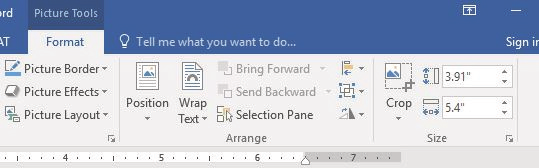
\includegraphics[width=\maxwidth{.95\linewidth}]{gfx/ch04_fig46}
	\caption{Paste Picture in Word}
	\label{04:fig46}
\end{figure}

Unfortunately, the picture is so big that it overlaps the next page. Use this procedure to change its size.

\begin{enumbox}
	\begin{enumerate}
		\item Click anywhere on the picture to activate it.
		\item Click \fmtButton{Picture Tools $ \Rightarrow $ Format $ \Rightarrow $ Size $ \Rightarrow $ Shape Width Down Arrow}. Continue to click the down arrow until the width of the picture is $ 5.4 $ inches (see Figure \ref{04:fig47}). As the width is reduced the height is automatically reduced. (The height should end up about $ 3.92 $ inches) (\fmtNewExcel{Excel 365} names the tab Picture Format.)
		\item To center the chart on the page, make sure the chart is activated and click \fmtButton{Home $ \Rightarrow $ Paragraph $ \Rightarrow $ Center}. 
		\item Save the document and close Word.
	\end{enumerate}
\end{enumbox}
	
\begin{figure}[H]
	\centering
	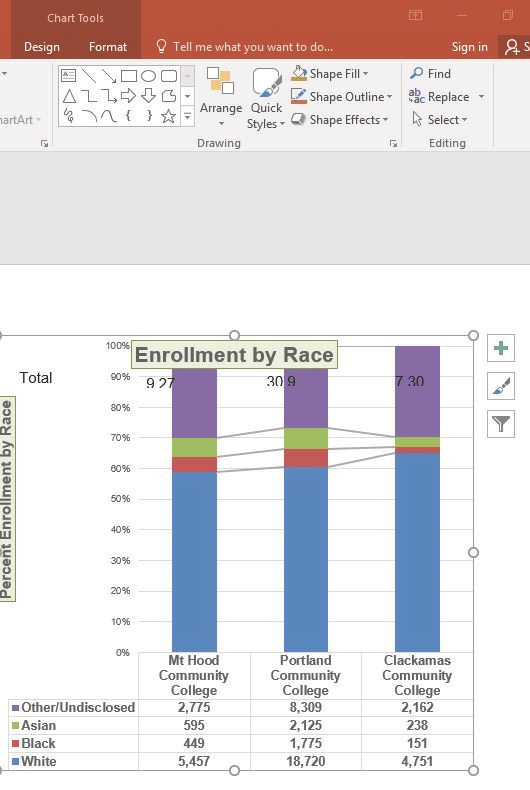
\includegraphics[width=\maxwidth{.75\linewidth}]{gfx/ch04_fig47}
	\caption{Changing the Size of a Picture in Word}
	\label{04:fig47}
\end{figure}

Figure \ref{04:fig48} shows the final appearance of the \textit{Enrollment by Race Source} chart pasted into a Word document. 

\begin{center}
	\begin{infobox}{Note}
		\textbf{Resizing Images}
		\\
		\\
		It is best to use either the \textit{Shape Width} or \textit{Shape Height} buttons to reduce the size of an embedded chart. Using either button automatically reduces both height and width in proper proportion. If the sizing handles are used, press and hold \fmtKeystroke{Shift}, then drag a corner sizing handle to keep the chart in proper proportion.
	\end{infobox}
\end{center}

\begin{figure}[H]
	\centering
	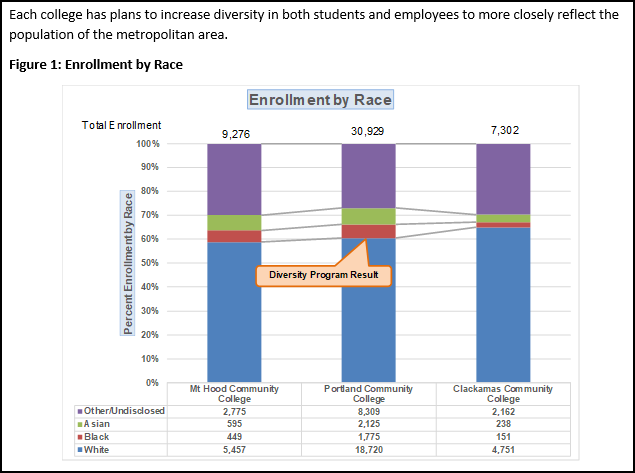
\includegraphics[width=\maxwidth{.95\linewidth}]{gfx/ch04_fig48}
	\caption{Final Appearance of Pasting a Chart Image into Word}
	\label{04:fig48}
\end{figure}

\begin{center}
	\begin{sklbox}{Skill Refresher}
		\textbf{Pasting a Chart Image into Word}
		\\
		\begin{itemize}
			\setlength{\itemsep}{0pt}
			\setlength{\parskip}{0pt}
			\setlength{\parsep}{0pt}

			\item Activate an Excel chart and click \textit{Home $ \Rightarrow $ Copy}.
			\item Click on the location in the Word document where the Excel chart will be pasted.
			\item Click \textit{Home $ \Rightarrow $ Paste Down Arrow $ \Rightarrow $ Picture}.
			\item Click \textit{Picture Tools $ \Rightarrow $ Format}. Resize the picture by clicking the up or down arrow on the \textit{Shape Width} or \textit{Shape Height} buttons.
			
		\end{itemize}
	\end{sklbox}
\end{center}

\subsection{Pasting a Linked Chart Image into PowerPoint}

This exercise requires two files:

\begin{itemize}
	\item The Excel spreadsheet used in this chapter: \textit{CH4-Charting}. (Note: this section continues the previous exercise. Students who only need to complete this section can open \textit{CH4-Charting Solution 1\_2} to start where the previous exercise ended.)
	\item A PowerPoint file: \textit{CH4-Diversity}
\end{itemize}

Microsoft PowerPoint is perhaps the most used tool for delivering live presentations. The charts used in a live presentation are critical for efficiently delivering ideas to an audience. Like written documents, a wide range of presentations may require the explanation of quantitative data. This demonstration includes a PowerPoint slide that could be used in a presentation. The \textit{Enrollment by Race} chart will be pasted into this PowerPoint slide. However, a link will be established to the Excel file rather than pasting an image. As a result, if the chart in the Excel file is changed, it will be reflected in the PowerPoint file. The following steps explain how to link these two files.

\begin{enumbox}
	\begin{enumerate}
		\item Open \fmtWorksheet{CH4-Diversity.pptx} and save it as \fmtWorksheet{CH4-Diversity Presentation}. (Note: the student files include both a PowerPoint presentation and a Word document named Diversity. Be sure to open the PowerPoint presentation for this activity.) 
		\item Navigate to Slide $ 6 $ --- \textit{Diversity in Enrollment}. This is the slide where the linked chart will be placed.
		\item If needed, open the Excel file used in this chapter, \fmtWorksheet{CH4-Charting}. Click the \textit{Enrollment by Race} chart in the \fmtWorksheet{Enrollment by Race Chart} sheet to activate it.
		\item Click \fmtButton{Home $ \Rightarrow $ Copy Down Arrow $ \Rightarrow $ Copy} (\textit{NOT} Copy as Picture).
		\item Go back to \fmtWorksheet{CH4-Diversity Presentation} by clicking the file in the taskbar.
		\item Make sure Slide 6, \textit{Diversity in Enrollment}, is still active. Click on the outside edge of the empty \textit{Click to add text} box on the right to activate it.
		\item Click \fmtButton{Home $ \Rightarrow $ Paste Down Arrow} in the PowerPoint file.
		\item Hover over each of the Paste Options until \fmtButton{Keep Source Formatting \& Link Data (F)} is highlighted (see Figure \ref{04:fig49}). Select this option. This pastes an image of the Excel chart into the PowerPoint slide. In addition, a link is created so that any changes made to the chart (in Excel) appear on the PowerPoint slide.
	\end{enumerate}
\end{enumbox}
	
\begin{figure}[H]
	\centering
	\includegraphics[width=\maxwidth{.75\linewidth}]{gfx/ch04_fig49}
	\caption{Creating a Link to an Excel Chart in PowerPoint}
	\label{04:fig49}
\end{figure}

Next, the chart needs to be cleaned up a bit. First, apply a different chart style.

\begin{enumbox}
	\begin{enumerate}
		\item Click anywhere in the plot area of the column chart pasted into the PowerPoint slide. The same Chart Tools tabs found in Excel are displayed on the ribbon (see Figure \ref{04:fig50}).
		\item Click \fmtButton{Chart Tools Design $ \Rightarrow $ Chart Style $ \Rightarrow $ Style $ 8 $}. (\fmtNewExcel{Excel 365} named the tab \textit{Chart Design}.) This is the style with a dark brown background.
	\end{enumerate}
\end{enumbox}
	
\begin{figure}[H]
	\centering
	\includegraphics[width=\maxwidth{.85\linewidth}]{gfx/ch04_fig50}
	\caption{Selecting a New Chart Style}
	\label{04:fig50}
\end{figure}

Linking this chart caused trouble with the text boxes, so delete them.

\begin{enumbox}
	\begin{enumerate}
		\item Select each text box by hovering the mouse over the outside edge of the text box until it changes into a four-headed arrow, then click.
		\item Tap \fmtKeystroke{Delete}. Be sure that the insertion point is \textit{NOT} blinking inside the text box. If it is, the contents of the text box will be edited instead of deleting the complete text box.
		\item Reposition and resize the \textit{Diversity Program Result} callout box so the text is visible and the callout points to the top of the first data item for Portland Community College.
	\end{enumerate}
\end{enumbox}
	
The benefit of adding this chart to the presentation as a link is that it will automatically update when the data in the linked spreadsheet file is changed.

\begin{enumbox}
	\begin{enumerate}
		\item Return to the \fmtWorksheet{CH4-Charting} Excel file.
		\item Select the \fmtWorksheet{Enrollment Statistics} worksheet (the one with the Enrollment data). Change the value in cell \fmtLoc{D3} to $ 1000 $ to change the number of white students at Clackamas Community College to $ 1000 $. This change is not factual but is large enough to see the result in the linked charts.
		\item Select the \fmtWorksheet{Enrollment by Race Chart} worksheet. Notice how the chart has changed.
		\item Return to \fmtWorksheet{Diversity Presentation} by clicking the file in the taskbar.
		\item On Slide $ 6 $, notice that the chart was updated to reflect the change in enrollment (see Figure \ref{04:fig48}).
		\item If the chart has not changed, be sure that the chart is selected; click \fmtButton{Chart Tools Design $ \Rightarrow $ Chart Tools $ \Rightarrow $ Refresh Data}. (\fmtNewExcel{Excel 365} named the tab \textit{Chart Design}.) The change made in the Excel workbook is now reflected on the PowerPoint slide.
		\item If that still does not work, check to see if a ``normal'' link was created instead of a ``Paste'' Link. If so, delete the chart and follow the steps again from the beginning of this section.
		\item Return the changed number to its original value. Open the  \fmtWorksheet{CH4-Charting} Excel file.
		\item Select the \fmtWorksheet{Enrollment Statistics} worksheet (the one with the Enrollment data). Change the value in cell \fmtLoc{D3} to $ 4751 $, the original value.
		\item Save all files and close PowerPoint. The files will be submitted at the end of the next section.
	\end{enumerate}
\end{enumbox}

Figure \ref{04:fig51} shows the appearance of the PowerPoint slide after the Excel chart was added. 

\begin{figure}[H]
	\centering
	\includegraphics[width=\maxwidth{.95\linewidth}]{gfx/ch04_fig51}
	\caption{Final PowerPoint Slide}
	\label{04:fig51}
\end{figure}

\begin{center}
	\begin{sklbox}{Skill Refresher}
		\textbf{Pasting a Linked Chart Image into PowerPoint}
		\\
		\begin{itemize}
			\setlength{\itemsep}{0pt}
			\setlength{\parskip}{0pt}
			\setlength{\parsep}{0pt}
			
			\item Activate an Excel chart and click the \textit{Copy} button in the \textit{Home} tab of the ribbon.
			\item Click in the PowerPoint slide where the Excel chart will be pasted.
			\item Click the down arrow of the \textit{Paste} button in the \textit{Home} tab of the ribbon.
			\item Click the \textit{Keep Source Formatting \& Link Data} option from the drop-down list.
			\item Click the \textit{Refresh Data} button in the \textit{Design} tab of the ribbon to ensure any changes in the Excel file are reflected in the chart.
			
		\end{itemize}
	\end{sklbox}
\end{center}

\begin{center}
	\begin{infobox}{Integrity Check}
		\textbf{Refreshing Linked Charts in PowerPoint and Word}
		\\
		\\
		When creating a link to a chart in Word or PowerPoint, the data must be refreshed when there are changes in the Excel workbook. This is especially true if the changes are made in the Excel file prior to opening the Word or PowerPoint file that contains a link to a chart. To refresh the chart, make sure it is activated, then click \textit{Chart Tools Design $ \Rightarrow $ Chart Tools $ \Rightarrow $ Refresh Data}. Forgetting this step can result in old or erroneous data being displayed in the chart.
	\end{infobox}
\end{center}

\begin{center}
	\begin{tkwbox}{Key Take-Aways}
		\textbf{Using Excel Charts with Word or PowerPoint}
		\\
		\begin{itemize}
			\setlength{\itemsep}{0pt}
			\setlength{\parskip}{0pt}
			\setlength{\parsep}{0pt}

			\item When pasting an image of an Excel chart into a Word document or PowerPoint file, use the \textit{Picture} option from the \textit{Paste} drop-down list of options to make it act as an image. Note that if the underlying data is updated the picture is not changed if it has been pasted as an image.
			\item When creating a link to a chart in Word or PowerPoint, the data may need to be refreshed if changes are made in the originating spreadsheet. 
					
		\end{itemize}
	\end{tkwbox}
\end{center}

\begin{center}
	\begin{infobox}{Integrity Check}
		\textbf{Severed Link?}
		\\
		\\
		When creating a link to an Excel chart in Word or PowerPoint, the Excel workbook must stay in its original location on the computer or network. If the workbook is moved or deleted, an error message will be generated when the link in the Word or PowerPoint file is updated. An error is also generated if the Excel workbook is saved on a network drive that the computer cannot access. These errors occur because the link to the Excel workbook has been severed. Therefore, if a USB drive is being used for a presentation then all the linked Excel workbooks must be moved to the USB drive before establishing the Word or PowerPoint link.
	\end{infobox}
\end{center}

\section{Preparing to Print}

\begin{center}
	\begin{objbox}{Learning Objectives}
		\begin{itemize}
			\setlength{\itemsep}{0pt}
			\setlength{\parskip}{0pt}
			\setlength{\parsep}{0pt}

			\item Review each worksheet in a workbook in Print Preview.
			\item Modify worksheets as needed to professionally print data and charts.
			
		\end{itemize}
	\end{objbox}
\end{center}

This section considers the worksheets created in the previous sections. Since these worksheets contain a combination of data and charts, there are specific things to watch for when they are printed.

A good starting point is to look at each worksheet in Print Preview in \textit{Backstage View}. Then make any necessary changes, such as changing the orientation and scaling, or moving charts around on the worksheet. To ensure that no worksheets are missed, review them in the order they appear in the tabs.

\subsection{Previewing Chart Sheets for Printing}

The first worksheet, \textit{Closing Prices}, is a chart sheet that contains no data; but it still needs to be reviewed in \textit{Print Preview}.

\begin{enumbox}
	\begin{enumerate}
		\item Open \fmtWorksheet{CH4-Charting} if it is not already open. (Note: this section continues the previous exercise. Students who only need to complete this section can open \textit{CH4-Charting Solution 1\_3} to start where the previous exercise ended.)
		\item Click on the \fmtWorksheet{Closing Prices} worksheet tab.
		\item Click \fmtButton{File $ \Rightarrow $ Print}.
		\item Notice that the chart will print on the entire page in Landscape orientation.
		\item There is nothing to change so close the print preview by clicking the arrow at the top left corner of the preview screen.
	\end{enumerate}
\end{enumbox}
	
\subsection{Printing Worksheets with Data and Charts}

The second worksheet (\textit{Stock Trend}) has data and two charts. The page setup will need some modification to print the data and the charts.

\begin{enumbox}
	\begin{enumerate}
		\item Click the \fmtWorksheet{Stock Trend} worksheet tab to open that worksheet.
		\item Click \fmtButton{File $ \Rightarrow $ Print}.
		\item Notice that this worksheet is currently printing on seven pages.
		\item Click through each page and note the following.
	
		\begin{itemize}
			\item The data is split between the first and third pages.
			\item The line chart starts on the first page, but part of it is also on the second page.
			\item The double-line chart starts on the third page and then finishes on the fifth page.
			\item The fourth and sixth pages are blank (or nearly blank).
			\item The last page has a column of seemingly random numbers.
		\end{itemize}
	
		\item Close the print preview by clicking the arrow at the top left corner of the preview screen.
	\end{enumerate}
\end{enumbox}
	
The first thing to do is remove the numbers appearing on page seven. To do this, hide the column where they are stored. It is essential to hide the column instead of deleting the numbers in case they are utilized elsewhere in the workbook.

\begin{enumbox}
	\begin{enumerate}
		\item Scroll to the right on the worksheet until the numbers in \fmtLoc{Column AH} are visible.
		\item Click anywhere in \fmtLoc{Column AH}.
		\item Click \fmtButton{Home$ \Rightarrow $ Cells $ \Rightarrow $ Format $ \Rightarrow $ Visibility $ \Rightarrow $ Hide \& Unhide $ \Rightarrow $ Hide Columns} (see Figure \ref{04:fig52}).
		
		\begin{figure}[H]
			\centering
			\includegraphics[width=\maxwidth{.95\linewidth}]{gfx/ch04_fig52}
			\caption{Hide Columns in Format Menu}
			\label{04:fig52}
		\end{figure}
			
		\item The visible column headings should now go from \fmtLoc{AG} to \fmtLoc{AI}.
		\item Click \fmtButton{File $ \Rightarrow $ Print}.
		\item Notice that there are now five pages. The data and charts are still splitting across multiple pages, but the numbers in \fmtLoc{Column AH} are no longer printing.
		\item Remain in \textit{Print Preview} for the next steps.
	\end{enumerate}
\end{enumbox}

The data is still split between Page $ 2 $ and Page $ 3 $, and the charts are splitting oddly. The first step to fixing these issues is to change the page orientation and scaling.

\begin{enumbox}
	\begin{enumerate}
		\item While still in \textit{Print Preview}, change the page orientation to \fmtButton{Landscape}.
		\item This puts all the data on one sheet, but the charts are still split between two pages.
		\item Change the page scaling to \fmtButton{Fit Sheet on One Page}.
		\item This fits everything on one page, but it is too small to be able to read.
		\item Change the page scaling back to \fmtButton{No Scaling}.
	\end{enumerate}
\end{enumbox}
	
The next thing to try is moving one, or both, of the charts. 

\begin{enumbox}
	\begin{enumerate}
		\item Close the print preview by clicking the arrow at the top left corner of the preview screen.
		\item Click \fmtButton{View $ \Rightarrow $ Workbook Views $ \Rightarrow $ Page Break Preview}. The screen should look like Figure \ref{04:fig53}. (Remember that the dotted blue lines indicate automatic page breaks.)
		\item Move the \textit{24 Month Comparison} (double-line) chart closer to the top of its page.
		\item Move the \textit{May 2014-2015 Trend for NASDAQ Sales Volume} (line chart) so that it is under the \textit{24 Month Comparison} chart.
		\item The link to the data source is still at the bottom of page $ 2 $ (in \fmtLoc{A50:A51}) so it needs to be moved to \fmtLoc{M31:M32}.
		\item The screen should look similar to Figure \ref{04:fig54}.
	\end{enumerate}
\end{enumbox}

\begin{figure}[H]
	\centering
	\includegraphics[width=\maxwidth{.95\linewidth}]{gfx/ch04_fig53}
	\caption{Page Break Preview before moving the charts in Step 3}
	\label{04:fig53}
\end{figure}

\begin{figure}[H]
	\centering
	\includegraphics[width=\maxwidth{.95\linewidth}]{gfx/ch04_fig54}
	\caption{Page Break Preview after moving the charts and text}
	\label{04:fig54}
\end{figure}

The data source link text should not print on a separate page, but there is no room to move it onto the same page as the charts. To fix this, remove the automatic page break between the charts and the text in $ M31 $:$ M32 $.

\begin{enumbox}
	\begin{enumerate}
		\item Place the pointer on the horizontal blue dashed line (automatic page break) between the line chart and the Data Source link text.
		\item When the pointer changes to the double arrow (pointing up and down), drag the page break down into the gray area. This removes the page break.
		\item If the vertical automatic page break between \fmtLoc{Column L} and \fmtLoc{Column M} moves, drag it back between \fmtLoc{Column L} and \fmtLoc{Column M}. This will make it a solid blue line, which will no longer adjust automatically.
		\item The screen should now look like Figure \ref{04:fig55}.
	\end{enumerate}
\end{enumbox}
	
\begin{figure}[H]
	\centering
	\includegraphics[width=\maxwidth{.95\linewidth}]{gfx/ch04_fig55}
	\caption{Page Break Preview after removing a page break}
	\label{04:fig55}
\end{figure}

Now complete one final check of this worksheet in Print Preview.

\begin{enumbox}
	\begin{enumerate}
		\item Click \fmtButton{View $ \Rightarrow $ Workbook Views $ \Rightarrow $ Normal}.
		\item Click \fmtButton{File $ \Rightarrow $ Print}.
		\item Page $ 1 $ should contain just the data and page $ 2 $ should have both charts and the Data Source link text.
		\item Close the print preview by clicking the arrow at the top left corner of the preview screen.
		\item Save the \fmtWorksheet{CH4-Charting} workbook.
	\end{enumerate}
\end{enumbox}
	
\subsection{Preview Remaining Worksheets for Printing}

There are four remaining worksheets to be reviewed. Some of them will need minor changes, and some will not need any changes. Print preview each one and make the changes specified.

\begin{enumbox}
	\begin{enumerate}
		\item \fmtWorksheet{All Excel Classes}: this is a chart sheet, so it should not need any changes.
		\item \fmtWorksheet{Grade Distribution}: the chart is split across two pages. Fix this by changing the orientation (Landscape) and scaling (Fit Sheet on One Page).
		\item \fmtWorksheet{Enrollment by Race Chart}: this is a chart sheet, so it should not need any changes.
	\end{enumerate}
\end{enumbox}

\subsection{Printing a Chart Only}

Sometimes a worksheet may have both data and a chart, but only the chart should print. That is the case with the \textit{Enrollment Statistics} worksheet.

\begin{enumbox}
	\begin{enumerate}
		\item Switch to the \fmtWorksheet{Enrollment Statistics} worksheet.
		\item Click the pie chart to activate it.
		\item Click \fmtButton{File $ \Rightarrow $ Print}.
		\item Only the chart is printing. (If it shows the data printing along with the chart, exit print preview and be sure to select just the chart on the worksheet.)
		\item If needed, change the orientation to Landscape. This orientation looks better when printing just a chart.
		\item Exit print preview.
	\end{enumerate}
\end{enumbox}
	
\subsection{Hiding a Worksheet}

It is possible to hide an entire worksheet so it will not print, nor will anyone looking at the workbook see it. Remember that this is not a security feature since someone can unhide the sheet, but it makes it easier to focus on essential data and charts. For this section, hide the \textit{Enrollment by Race Chart} sheet.

\begin{enumbox}
	\begin{enumerate}
		\item Right-click on the \fmtWorksheet{Enrollment by Race Chart} tab.
		\item Select \fmtButton{Hide} from the menu that appears. The \fmtWorksheet{Enrollment by Race Chart} sheet should no longer be visible.
		\item To unhide the worksheet, right-click on any other worksheet tab and select Unhide from the menu. A list of hidden worksheets will be displayed. Select the \fmtWorksheet{Enrollment by Race Chart} and click \fmtButton{OK}.
		\item Save the \fmtWorksheet{CH4-Charting} workbook.
		\item Compare all workbooks with their self-check answer key: \fmtWorksheet{CH4-Charting Solution}, \fmtWorksheet{CH4-Diversity Report Solution}, and \fmtWorksheet{CH4-Diversity Presentation Solution}.
		\item Close and submit all three files (\fmtWorksheet{CH4-Charting}, \fmtWorksheet{CH4-Diversity Report}, and \fmtWorksheet{CH4-Diversity Presentation}) as directed by the instructor.
	\end{enumerate}
\end{enumbox}
	
\section{Chapter Practice}

Although Excel is primarily used in business and scientific applications, it is also valuable for other areas of study. Excel creates charts using historical, health, and social justice data in the following exercises.

\subsection{Charting Historical Data (Comprehensive Review)}

Excel is an excellent tool for helping to display historical data. This exercise examines information on minimum wage data and life expectancy.

\subsubsection{Task1 – National Minimum Wage in the Us – 1960-2014}

Since the beginning of the previous century, the United States has set a minimum wage to set a ``floor'' beneath which wages cannot fall. Most states have set minimum wages, but none are lower than the national minimum wage\footnote{To learn more about the national minimum wage, look at \url{https://en.wikipedia.org/wiki/Minimum_wage_in_the_United_States}.}.

\begin{enumbox}
	\begin{enumerate}
		\item Open the file named \fmtWorksheet{PR4-Data} and then Save As \fmtWorksheet{PR4-Historical Data}.
		\item On the \fmtWorksheet{Minimum Wage} worksheet, select \fmtLoc{B4:C60}.
		\item Click \fmtButton{Insert $ \Rightarrow $ Charts $ \Rightarrow $ Recommended Chart}. \textit{Recommended Charts} allows users to first see how selected data would be represented on a variety of chart types before committing to a particular type of chart. Being able to see the data as it would look in a variety of charts helps when selecting the kind of chart that best matches the data. It does a particularly good job when using dates or years as labels, though sometimes Excel gets confused and thinks that dates are part of the data instead of labels.
		\item Select the first \textit{Line Chart} and tap \fmtButton{OK}.
		\item The line chart is created in the \fmtWorksheet{Minimum Wage} worksheet.
		\item Resize the chart using the following values. For each side of the chart, press and hold \fmtKeystroke{Alt}, then left-click and drag the resize handle on the chart to make it ``lock into'' position.
	
		\begin{table}[H]
		\rowcolors{1}{}{tablerow} % zebra striping background
		\captionsetup{labelformat=empty} % kill the label and caption area
		{\small
			%\fontsize{8}{10} \selectfont %Replace small for special font size
			\begin{longtable}{R{0.75in}L{1.50in}} %Left-aligned, Max width: 4.25in
				\textbf{Chart Side} & \textbf{Locked To} \endhead
				\hline
				Top & Top of \fmtLoc{Row 4}\\
				Left & Left of \fmtLoc{Column E}\\
				Bottom & Bottom of \fmtLoc{Row 20}\\
				Right & Right of \fmtLoc{Column M}\\
			\end{longtable}
		} % End small
		\end{table}
	
		\item Click the chart title once and then click in front of the first letter. A blinking cursor appears in front of the letter. Type the following in front of the first letter in the chart title: \fmtTyping{U.S. National} (be sure to leave a space after the word \textit{National}).
		\item While the chart is still selected, click \fmtButton{Chart Tools Design $ \Rightarrow $ Chart Styles}. (\fmtNewExcel{Excel 365} named the tab \textit{Chart Design}.) If necessary, tap \fmtButton{More} to see the available styles.
		\item Float the cursor over the available styles to see how each will affect the chart. Select Style Four, which fills a vertical stripe pattern under the line.
		\item The years across the X-Axis are a little hard to read. Select the labels so there is a box surrounding the list of years. 
		\item Click \fmtButton{Home $ \Rightarrow $ Alignment $ \Rightarrow $ Orientation $ \Rightarrow $ Angle Counterclockwise}.
		\item Click \fmtLoc{A1} to select that cell.
		\item Prepare the \fmtWorksheet{Minimum Wage} worksheet for printing by changing the scaling on the \textit{Print Preview} screen to \textit{Fit Sheet on One Page}.
		\item Close the print preview by clicking the arrow at the top left corner of the preview screen.
	\end{enumerate}
\end{enumbox}

\subsubsection{Task2 – Oregon: Projected Life Expectancy at Birth}

In the past $ 40 $ years, between $ 1970 $ and $ 2010 $, life expectancy for Oregon men improved by $ 8.7 $ years and for women by $ 5.5 $ years. Oregon's life expectancy has remained slightly higher than the U.S. average. The life expectancy will continue to improve for both men and women; however, the gain for men has been outpacing the gain for women. Consequently, the difference between men's and women's life expectancies has continued to shrink\footnote{This data was found at \url{https://www.oregon.gov/das/OEA/Documents/OR_pop_trend2012.pdf}.}.

\begin{enumbox}
	\begin{enumerate}
		\item On the \fmtWorksheet{Life Expectancy} sheet, select \fmtLoc{A5:B11}
		\item Tap \fmtKeystroke{F11} to automatically create a column chart on a new worksheet. (\textit{NOTE: If the Instant Chart feature does not work, then manually create a column chart.})
		\item Double click the chart sheet tab name and change it to \fmtTyping{Men}.
		\item Take a good look at this chart. It is not what was expected. Excel has made a mistake and charted the \textit{Birth Year} information as though it was data, instead of using it to label the Y-Axis.
		\item Click the chart to activate it.
		\item Click \fmtButton{Chart Tools Design $ \Rightarrow $ Data $ \Rightarrow $ Select Data}. (\fmtNewExcel{Excel 365} named the tab \textit{Chart Design}.) This opens the \textit{Select Data Source} dialog box. The box at the top reports the selected range, which looks fine. 
	\end{enumerate}
\end{enumbox}
		
The \textit{Legend Entries} in the large box on the left side of the \textit{Select Data Source} box need to be corrected. Also, the \textit{Horizontal Axis Labels} are just a series of default numbers, but they should be the range that contains the years.

\begin{enumbox}
	\begin{enumerate}
		\item In the \textit{Legend Entries}, click in the small box in front of \fmtButton{Birth Year} to remove the check mark. This will remove the \textit{Birth Year} as a data series on the chart.
		\item In the \textit{Horizontal (Category) Axis Labels} box, tap \fmtButton{Edit}. This will open the \textit{Axis Labels} dialog box. Tap \fmtButton{Select Range}.
		\item Navigate to the \fmtWorksheet{Life Expectancy} tab and select \fmtLoc{A6:A11}. After \fmtTyping{=’Life Expectancy’!$A$6:$A$11} is displayed in the box, tap \fmtButton{Select Range}. Tap \fmtButton{OK}. Tap \fmtButton{OK} a second time.
		\item Change the chart title to \fmtTyping{Life Expectancy for Oregon Men}.
		\item Remove the Legend from the bottom of the chart by right-clicking on it and selecting \fmtButton{Delete} from the context menu.
		\item Return to the \textit{Life Expectancy} tab and select \fmtLoc{A5:A11}, \fmtLoc{C5:C11} (Select the first range, press and hold \fmtKeystroke{Ctrl}, then select the second range.
		\item Repeat the above steps to create a matching chart for \fmtTyping{Life Expectancy for Oregon Women}.
		\item Return to the \textit{Life Expectancy} tab and select \fmtLoc{A5:D11}.
		\item Use the \fmtButton{Recommended Charts} tool to create a line chart (it will be the first option).
		\item Change the \textit{Chart Title} to \fmtTyping{Oregon: Projected Life Expectancy at Birth}.
		\item The green line across the bottom of the chart represents the difference between men's and women's life expectancy, but it is not helpful as it is. Right-click on the green line to open the context menu. Select \fmtButton{Format Data Series}. Select the radio button in the \textit{Format Data Series} pane in front of \fmtButton{Secondary Axis} under the \fmtButton{Series Options} tab.
		\item Close the \textit{Format Data Series} pane.
		\item Add a text box that explains the \textit{Difference} calculation. While the chart is still selected:
		
		\begin{itemize}
			\item Click \fmtButton{Insert $ \Rightarrow $ Text $ \Rightarrow $ Text Box}.
			\item Notice that the cursor has turned into a cross hair (thin black plus sign)
			\item Click once in the lower-left corner of the chart, near $ 0.0 $ on the Y-Axis to create a text box.
			\item Type the following into the text box: \fmtTyping{Difference = Female life expectancy minus male}. Tap \fmtKeystroke{Enter} after the word \textit{life} to create a two-line entry. 
			\item Move or resize the text box as desired.
		\end{itemize}
		
		\item Move or resize the chart, so it is no longer on top of the spreadsheet data.
		\item Click \fmtButton{Chart Tools Design $ \Rightarrow $ Chart Styles} and select the first style. (\fmtNewExcel{Excel 365} named the tab \textit{Chart Design}.)
		\item Preview the \fmtWorksheet{Life Expectancy} worksheet in \textit{Print Preview} and make any necessary changes to ensure the entire worksheet is visible.
		\item Save the \fmtWorksheet{PR4-Historical Data} workbook.
		\item Compare the worksheet with the self-check answer key (\fmtWorksheet{PR4-Historical Data Solution}) and then close and submit the \fmtWorksheet{PR4-Historical Data} workbook as directed by the instructor.
		
	\end{enumerate}
\end{enumbox}
	
\section{Scored Assessment}

\subsection{Charting Social Justice Data (Comprehensive Review)}

\subsubsection{Task 1 International Incarceration Rates}

\begin{enumbox}
	\begin{enumerate}
		\item Open the file named \fmtWorksheet{SC4-Data} and then Save As \fmtWorksheet{SC4-Social Justice}.
		\item On the \fmtWorksheet{International} tab, use a function in cell \fmtLoc{D20} to find the average of the \textit{Individuals Incarcerated} data.
		\item Create a bar chart that looks like Figure \ref{04:fig56}:
	\end{enumerate}
\end{enumbox}
	
\begin{figure}[H]
	\centering
	\includegraphics[width=\maxwidth{.95\linewidth}]{gfx/ch04_fig56}
	\caption{International Incarceration Rates}
	\label{04:fig56}
\end{figure}

\begin{enumbox}
	\begin{enumerate}
		\item Move and or resize the chart so that it does not cover any of the data.
		\item In cell \fmtLoc{A25} write a brief note explaining why a bar (or column) chart is a better choice for this data than a pie chart.
		\item Set the \textit{Print Area} so that everything prints, except for the explanation that was added in cell \fmtLoc{A25}.
		\item Preview the \fmtWorksheet{International} worksheet in \textit{Print Preview} and make any changes needed to print professionally on one page.
	\end{enumerate}
\end{enumbox}

\subsubsection{Task 2 Disenfranchisement Rate}

Felony disenfranchisement is excluding people from voting due to a felony conviction. Jurisdictions vary as to whether they make such disfranchisement permanent or restore suffrage after a person has served a sentence or completed parole or probation. Affected individuals suffer ``collateral consequences,'' including loss of access to jobs, housing, and other facilities.

Opponents have argued that such disfranchisement restricts and conflicts with principles of universal suffrage. It can affect civic and communal participation in general\footnote{For more information about disenfranchisement, see \url{https://en.wikipedia.org/wiki/Felony_disenfranchisement}.}.

\begin{enumbox}
	\begin{enumerate}
		\item On the \fmtWorksheet{Disenfranchisement Rate} sheet, use the \fmtButton{Recommended Charts} tool to create the three charts illustrated in Figures \ref{04:fig57}, \ref{04:fig58}, and \ref{04:fig59}. 
		\item Put each chart on its own individual sheet rather than an object in a spreadsheet.
		\item Be sure that \textit{years} are used as labels on the horizontal axis instead of numbers like $ 1 $, $ 2 $, $ 3 $. 
		\item Format the Washington and Oregon charts so the maximum for the left vertical axis is $ 20000 $ and the right vertical axis is $ .20 $. 
		\item Edit the text of the \textit{Chart Titles} on all three charts and format the title font: Arial, bold, 18pt.
	\end{enumerate}
\end{enumbox}
	
\begin{figure}[H]
	\centering
	\includegraphics[width=\maxwidth{.95\linewidth}]{gfx/ch04_fig57}
	\caption{Felony Disenfranchisement Rate Washington}
	\label{04:fig57}
\end{figure}

\begin{figure}[H]
	\centering
	\includegraphics[width=\maxwidth{.95\linewidth}]{gfx/ch04_fig58}
	\caption{Felony Disenfranchisement Rate Oregon}
	\label{04:fig58}
\end{figure}

\begin{figure}[H]
	\centering
	\includegraphics[width=\maxwidth{.95\linewidth}]{gfx/ch04_fig59}
	\caption{Comparison of Oregon and Washington}
	\label{04:fig59}
\end{figure}

\begin{enumbox}
	\begin{enumerate}
		\item Preview the worksheet(s) in Print Preview and make any necessary changes for professional printing.
		\item Save and close the \fmtWorksheet{SC4-Social Justice} workbook. 
		\item Submit the \fmtWorksheet{SC4-Social Justice} workbook as directed by the instructor.
	\end{enumerate}
\end{enumbox}